\chapter{Metodología aplicada}

En este capítulo se describe la metodología seguida para el desarrollo del proyecto, 
desde la documentación del proyecto, la caracterización del material, el análisis por 
elemento finito, el análisis experimental, y cada una de las etapas necesarias para 
la conclusión y consecución de los objetivos planteados. En la figura \ref{fig:diagrama_metodologia} 
se muestra un esquema de las etapas del desarrollo del proyecto y en las secciones 
subsiguientes se describen de manera más amplia las actividades que implica cada una de ellas.

\begin{center}
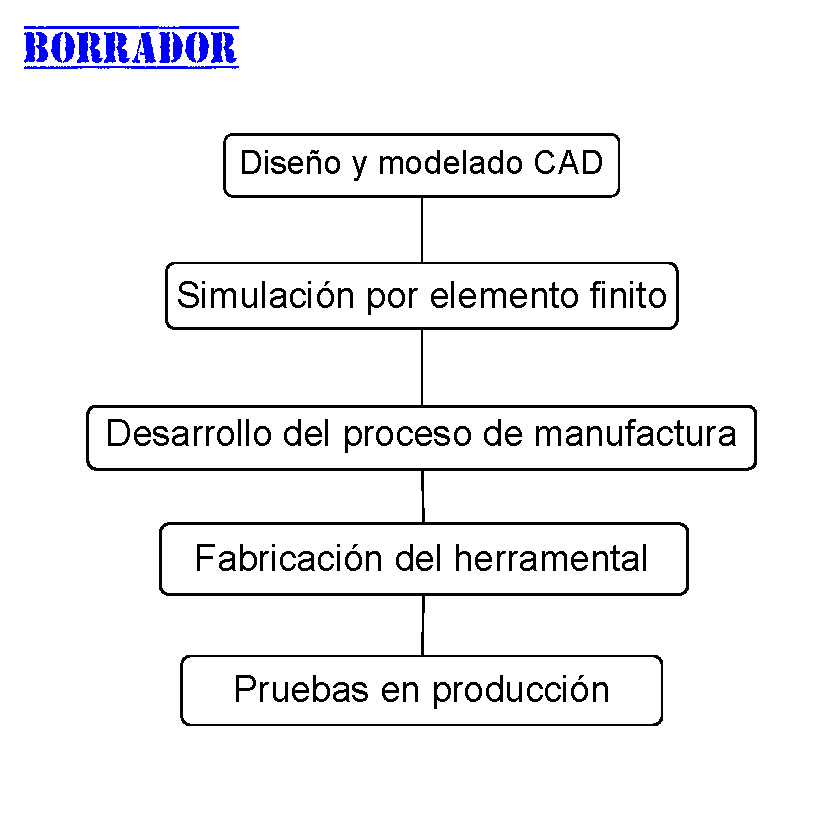
\includegraphics[width=0.75\textwidth]{src/ch3/diagrama_metodologia.pdf}
\captionof{figure}{Metodología del proyecto}
\label{fig:diagrama_metodologia}
\end{center}

\section{Consulta de fuentes de información}

En esta etapa inicial del proyecto se consultaron diversas fuentes de información 
relacionadas con los procesos de manufactura, específicamente los procesos 
de formado de hojas metálicas y operaciones de troquelado. Se buscó también información 
referente a la simulación por elementos finitos de operaciones que involucran 
deformación plástica, con la finalidad de conocer los tipos de análisis y definir 
el más conveniente para el caso. \\

Se consultó información relativa al estado del arte en artículos y/o publicaciones, 
sobre procesos de formado de manera general y para operaciones de doblado similares a la 
de este proyecto, es decir, aquellas que involucran una deformación sucesiva en UO. 
Todo esto se buscó en las principales bases de datos de contenido científico tales 
como Springer, Thomson, Elsevier, Scielo, Redalyc, así como en las bibliotecas 
digitales de diversas universidades hispanas y anglosajonas que proporcionan una 
cantidad considerable de trabajos de tesis, además de una revisión general en 
Google Scholar, que refiere e indexa la mayor parte del contenido de carácter científico 
y/o académico.

\section{Caracterización del material}

Cuando se requiere conocer las propiedades mecánicas de un material en ingeniería, se utilizan ensayos 
normalizados. En este caso se hace necesario obtener la curva esfuerzo-deformación del 
acero AISI 1018, misma que se utiliza como dato de entrada para la definición del ma
    terial 
en el software de simulación utilizado. Para obtener el comportamiento esfuerzo-deformación 
de un metal se utiliza un ensayo de tensión uniaxial descrito en la norma ASTM-E8. ~\cite{ASTME8} \\

Del ensayo de tensión se obtuvieron los datos agrupados en la curva de la figura \ref{fig:material_curve}, 
en la cual se muestra, además, la curva esfuerzo-deformación verdadera calculada mediante las ecuaciones 
\ref{eq:true_stress} y \ref{eq:true_strain}.

\begin{center}
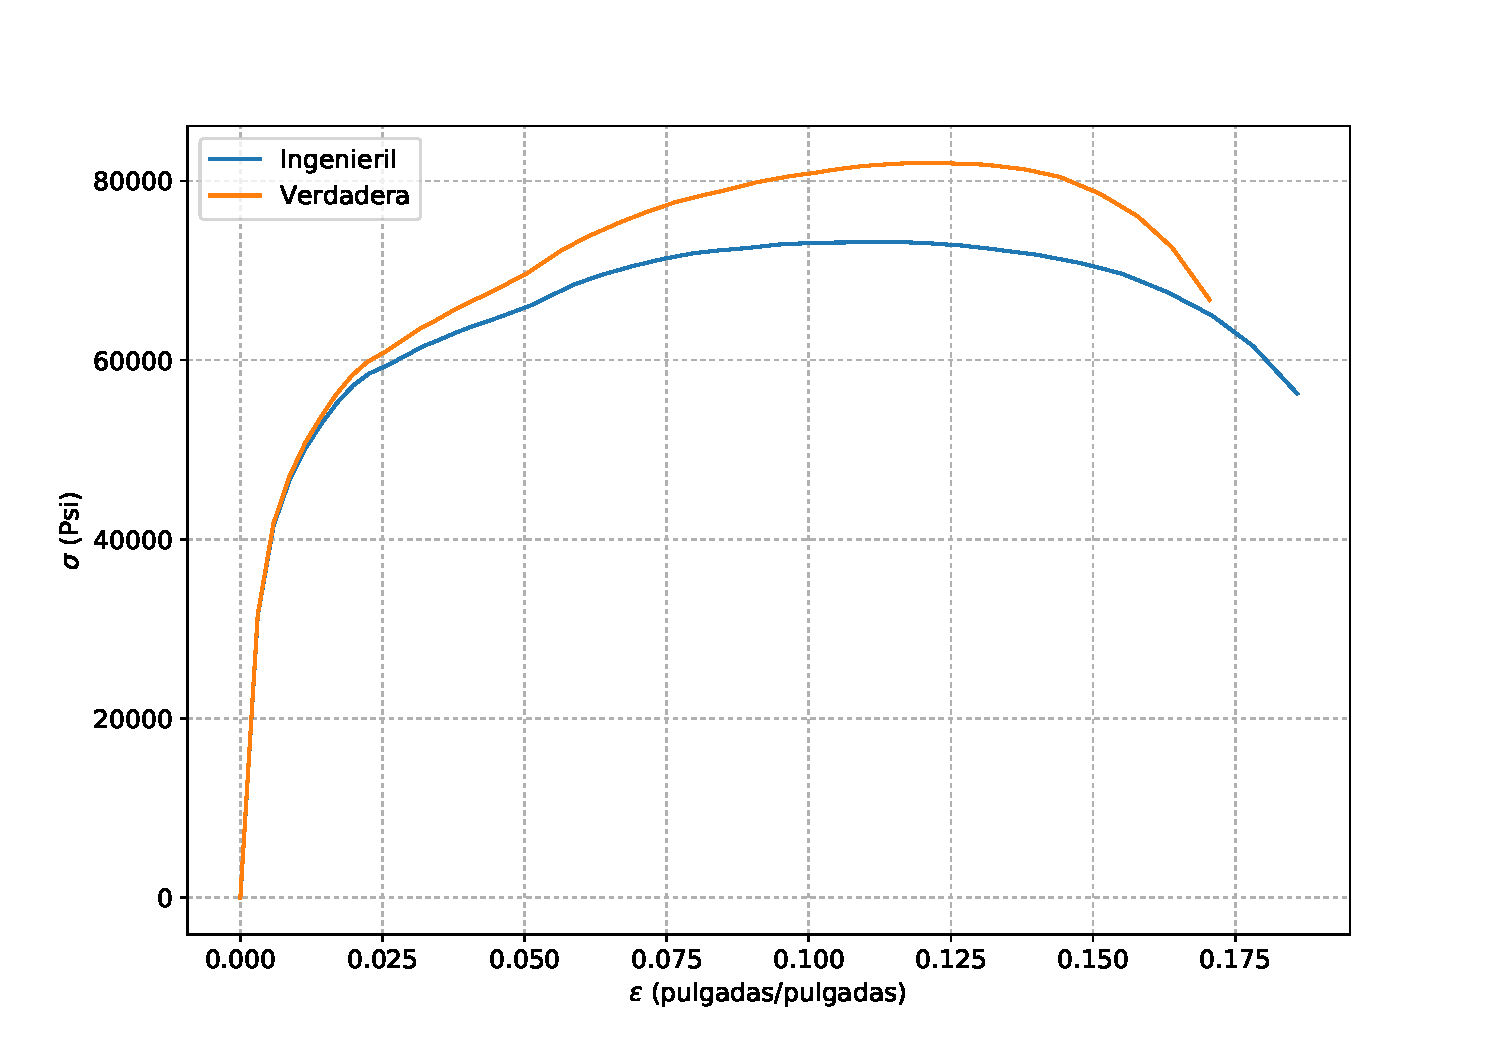
\includegraphics[scale=0.6]{src/ch3/material_curve.pdf}
\captionof{figure}{Curvas de esfuerzo-deformación, ingenieril y verdadera, del acero AISI 1018}
\label{fig:material_curve}
\end{center}

\section{Análisis por elementos finitos}

Como se describió en la sección \ref{subsec:implementacion-fem}, el análisis por elementos 
finitos en problemas de ingeniería es un proceso iterativo, en el que normalmente hay que ajustar 
algunos parámetros e ir revisando que los resultados obtenidos sean, al menos en principio, 
coherentes o se encuentren dentro de un rango esperado. \\

En el esquema mostrado en la figura \ref{fig:fem_diagram} se observa una metodología generalizada 
para un análisis por elementos finitos, partiendo desde el planteamiento de las 
ecuaciones diferenciales que gobiernan el problema. Cuando se utiliza un software 
de simulación, estos normalmente incorporan un entorno integrado que 
proporciona y facilita el desarrollo de un modelo de elementos finitos a partir 
de las geometrías involucradas, debido a esto, el proceso para el análisis por elementos 
finitos involucra algunas cuestiones como las que se muestran en el diagrama de 
la figura \ref{fig:metodologia_analisis_fem}, el cual sería más acorde con 
el proceso de análisis realizado en este caso.

\begin{center}
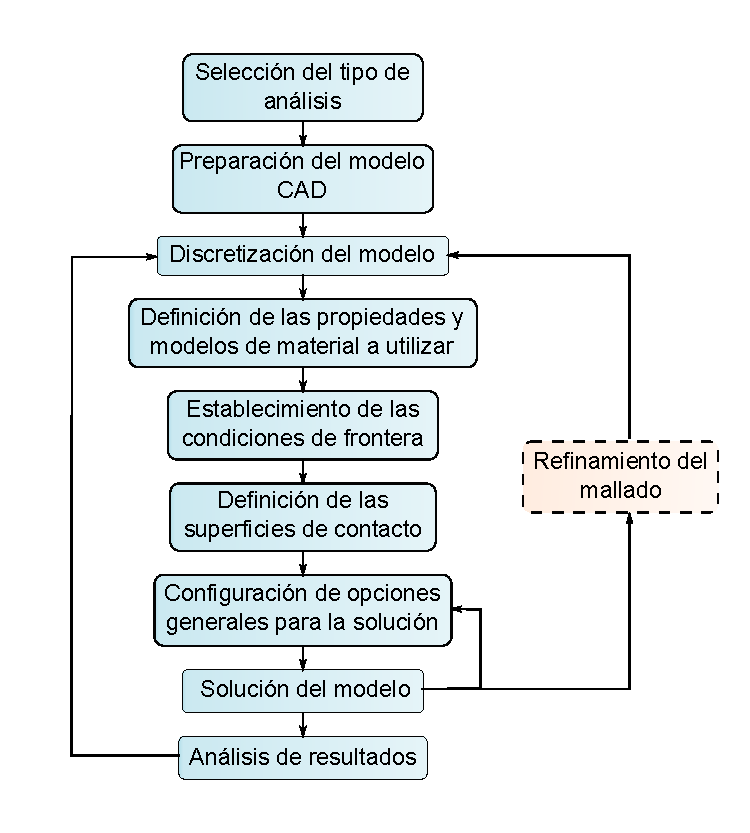
\includegraphics[width=0.65\textwidth]{src/ch3/metodologia_analisis_fem.pdf}
\captionof{figure}{Metodología para el análisis por elemento finito}
\label{fig:metodologia_analisis_fem}
\end{center}

\subsection{El proceso a simular}

En el capítulo \ref{ch:marco_de_referencia} se ha descrito someramente el proceso de formado que se requiere 
simular. Ahora, en lo subsiguiente, se detallan en mayor grado las características 
relativas al proceso, materiales utilizados y condiciones de operación que influyen en este. \\

El tubo interior mostrado en la figura \ref{fig:ti_rb131} se utiliza en un buje como 
el mostrado en la figura \ref{fig:buje_rb131}, el cual forma parte de un sistema de muelles 
parabólicas similar al de \ref{fig:muelle_parabolica}.

\begin{figure}[!h]
\centering
\begin{subfigure}[t]{0.35\textwidth}
\centering
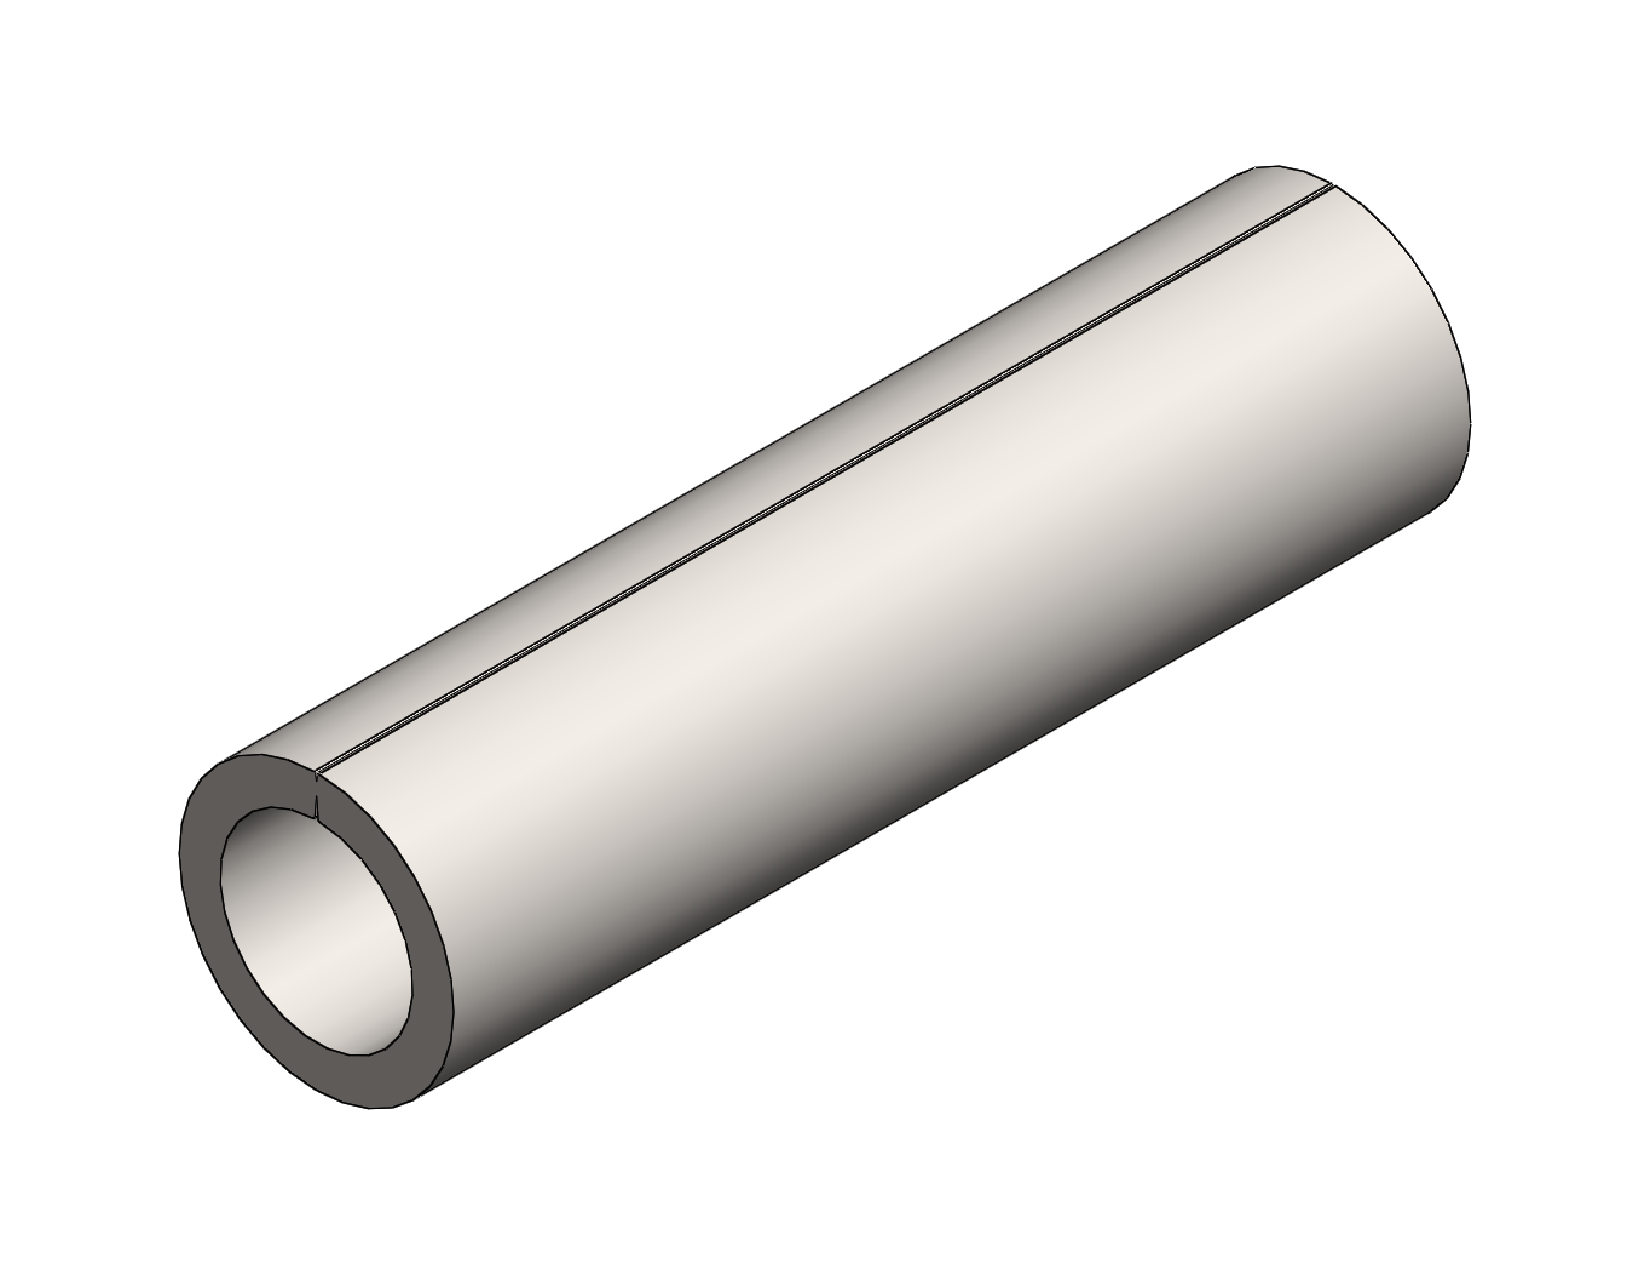
\includegraphics[width=\textwidth]{src/ch3/ti_rb131.pdf}
\caption{}
\label{fig:ti_rb131}
\end{subfigure}
~  
\begin{subfigure}[t]{0.35\textwidth}
\centering
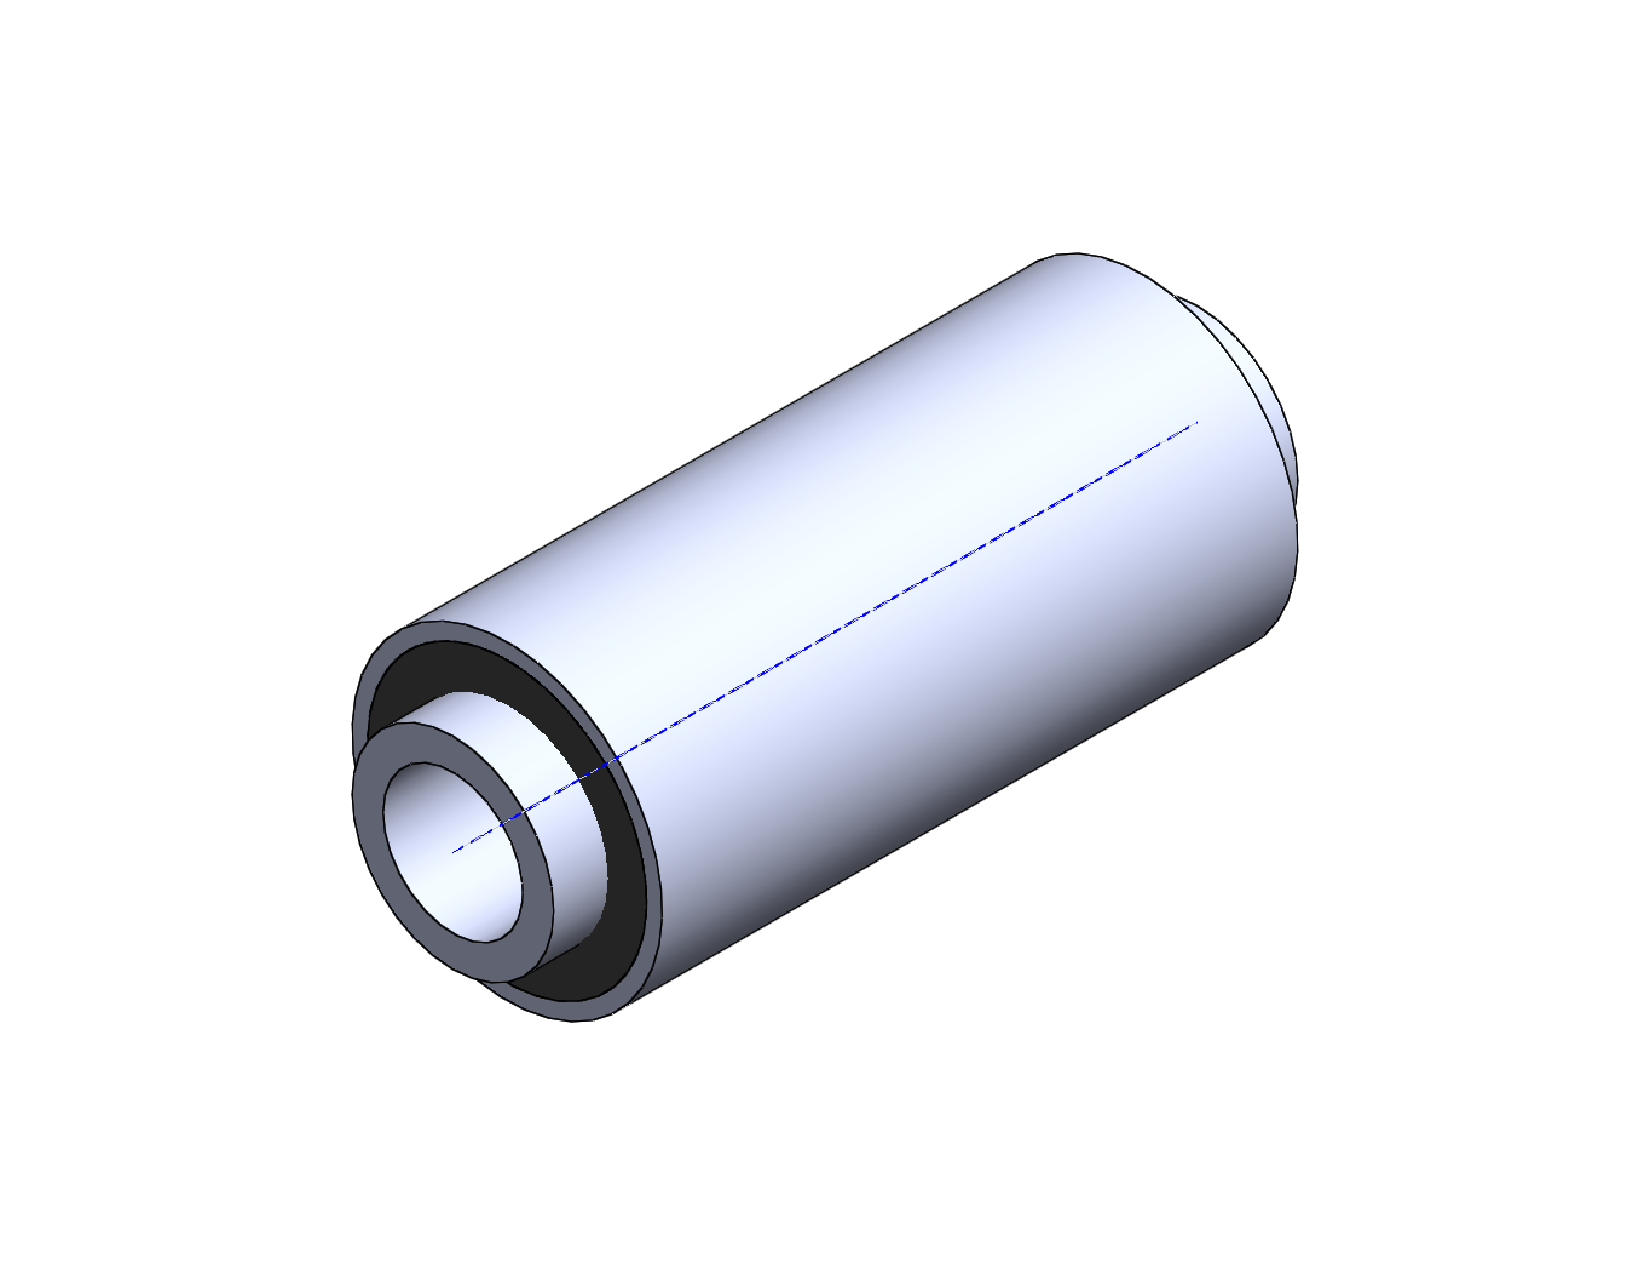
\includegraphics[width=\textwidth]{src/ch3/buje_rb131.pdf}
\caption{}
\label{fig:buje_rb131}
\end{subfigure}
\caption{a) Modelo CAD del tubo interior manufacturado por estampado b) Modelo CAD del buje RB-131}
\end{figure}


Para fabricar el tubo interior \ref{fig:ti_rb131} se utiliza un troquel compuesto o semiprogresivo 
de dos etapas, a saber: un doblado en U y un cerrado o doblado en O, mismo cuyo modelo CAD se muestra 
en la figura \ref{fig:troquel}. El troquel tiene como materia de entrada una placa metálica 
(\textit{blank}) rectangular de acero AISI 1018, con un largo de 3 in y un acho de 2.125 in, 
con un espesor de 0.12 in (ver figura \ref{fig:blank_inicial}). El \textif{blank} tiene además 
dos chaflanes en la dirección axial, sobre una de las caras, mismos que sirven para permitir un 
cierre de tubo adecuado.


\begin{center}
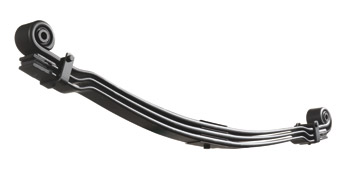
\includegraphics[scale=0.65]{src/ch3/muelle_parabolica.jpg}
\captionof{figure}{Muelle parabólica}
\label{fig:muelle_parabolica}
\end{center}


\begin{center}
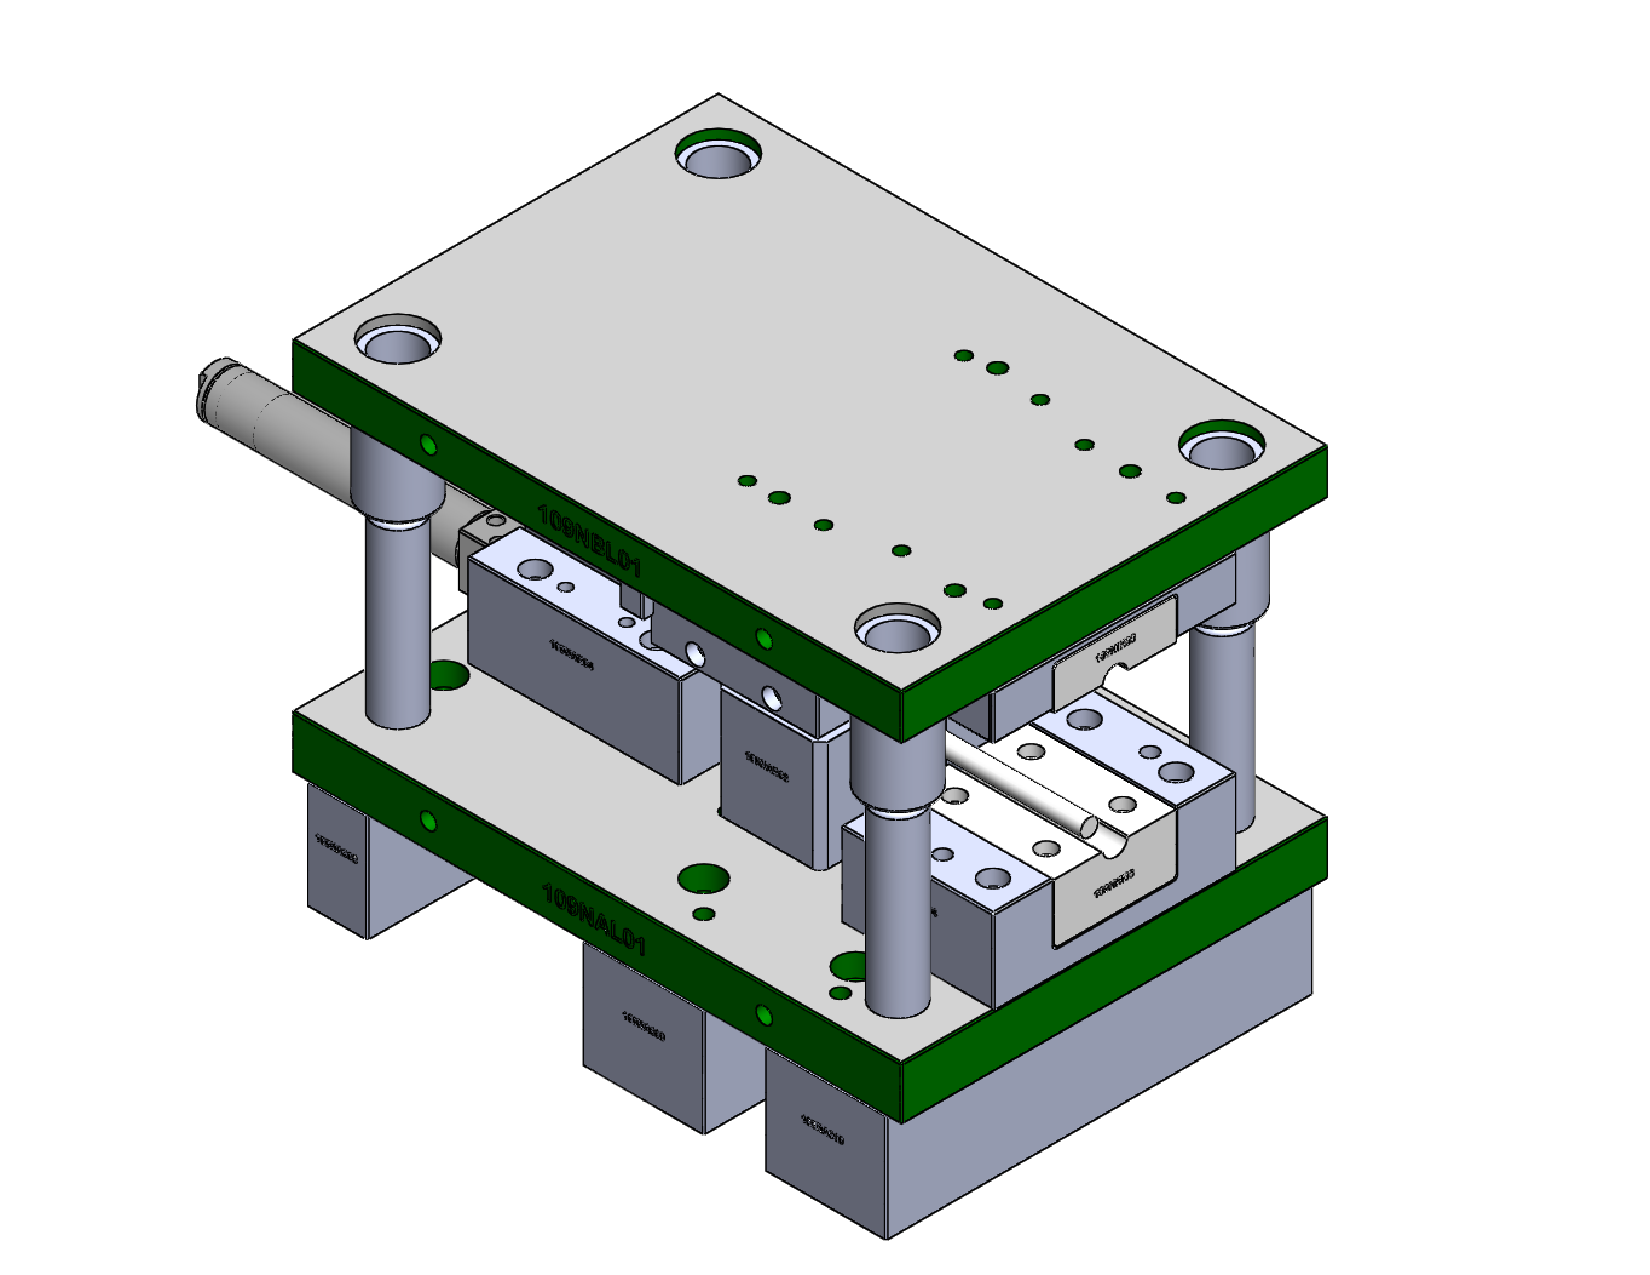
\includegraphics[scale=0.4]{src/ch3/troquel.pdf}
\captionof{figure}{Vista completa del troquel}
\label{fig:troquel}
\end{center}


\begin{figure}[!h]
\centering
\begin{subfigure}[t]{0.45\textwidth}
    \centering
    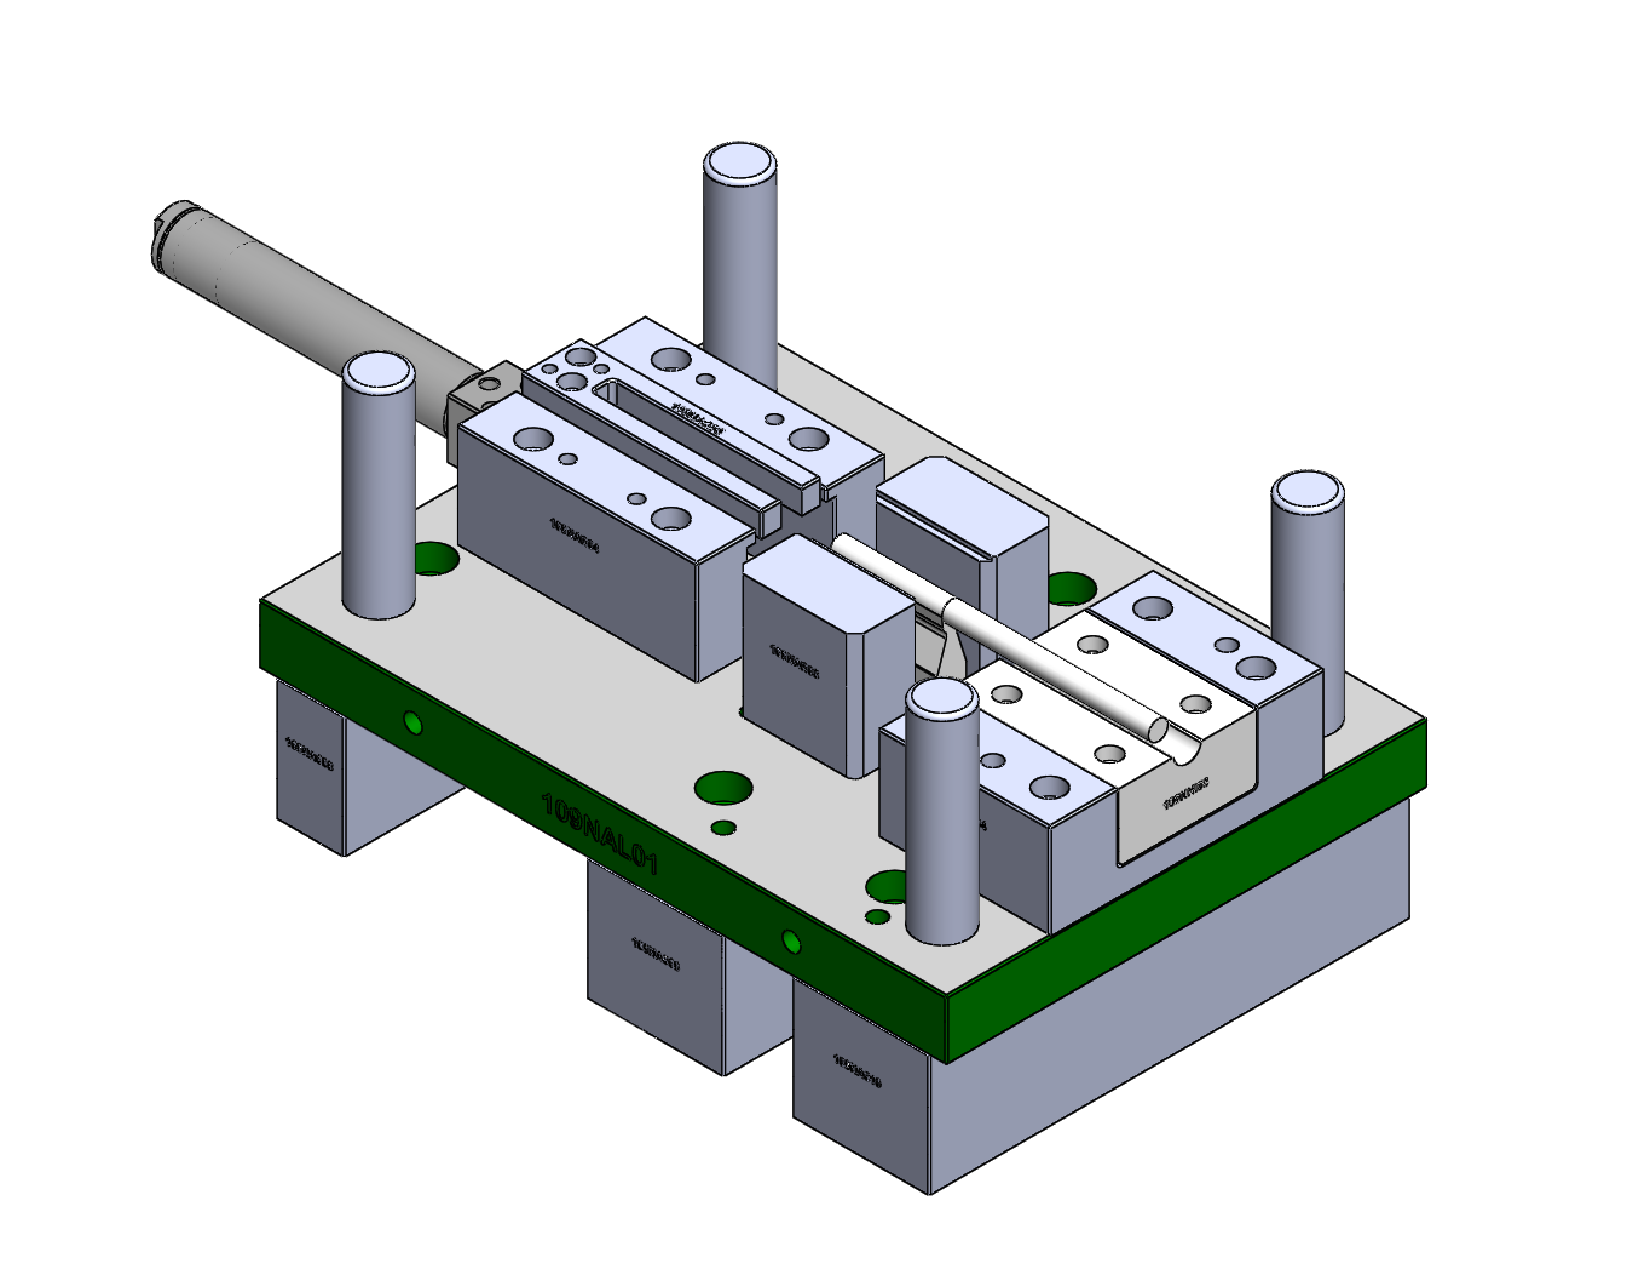
\includegraphics[width=\textwidth]{src/ch3/troquel_vista_inferior.pdf}
    \caption{}
    \label{fig:troquel_vista_inferior}
\end{subfigure}
~ 
\begin{subfigure}[t]{0.45\textwidth}
    \centering
    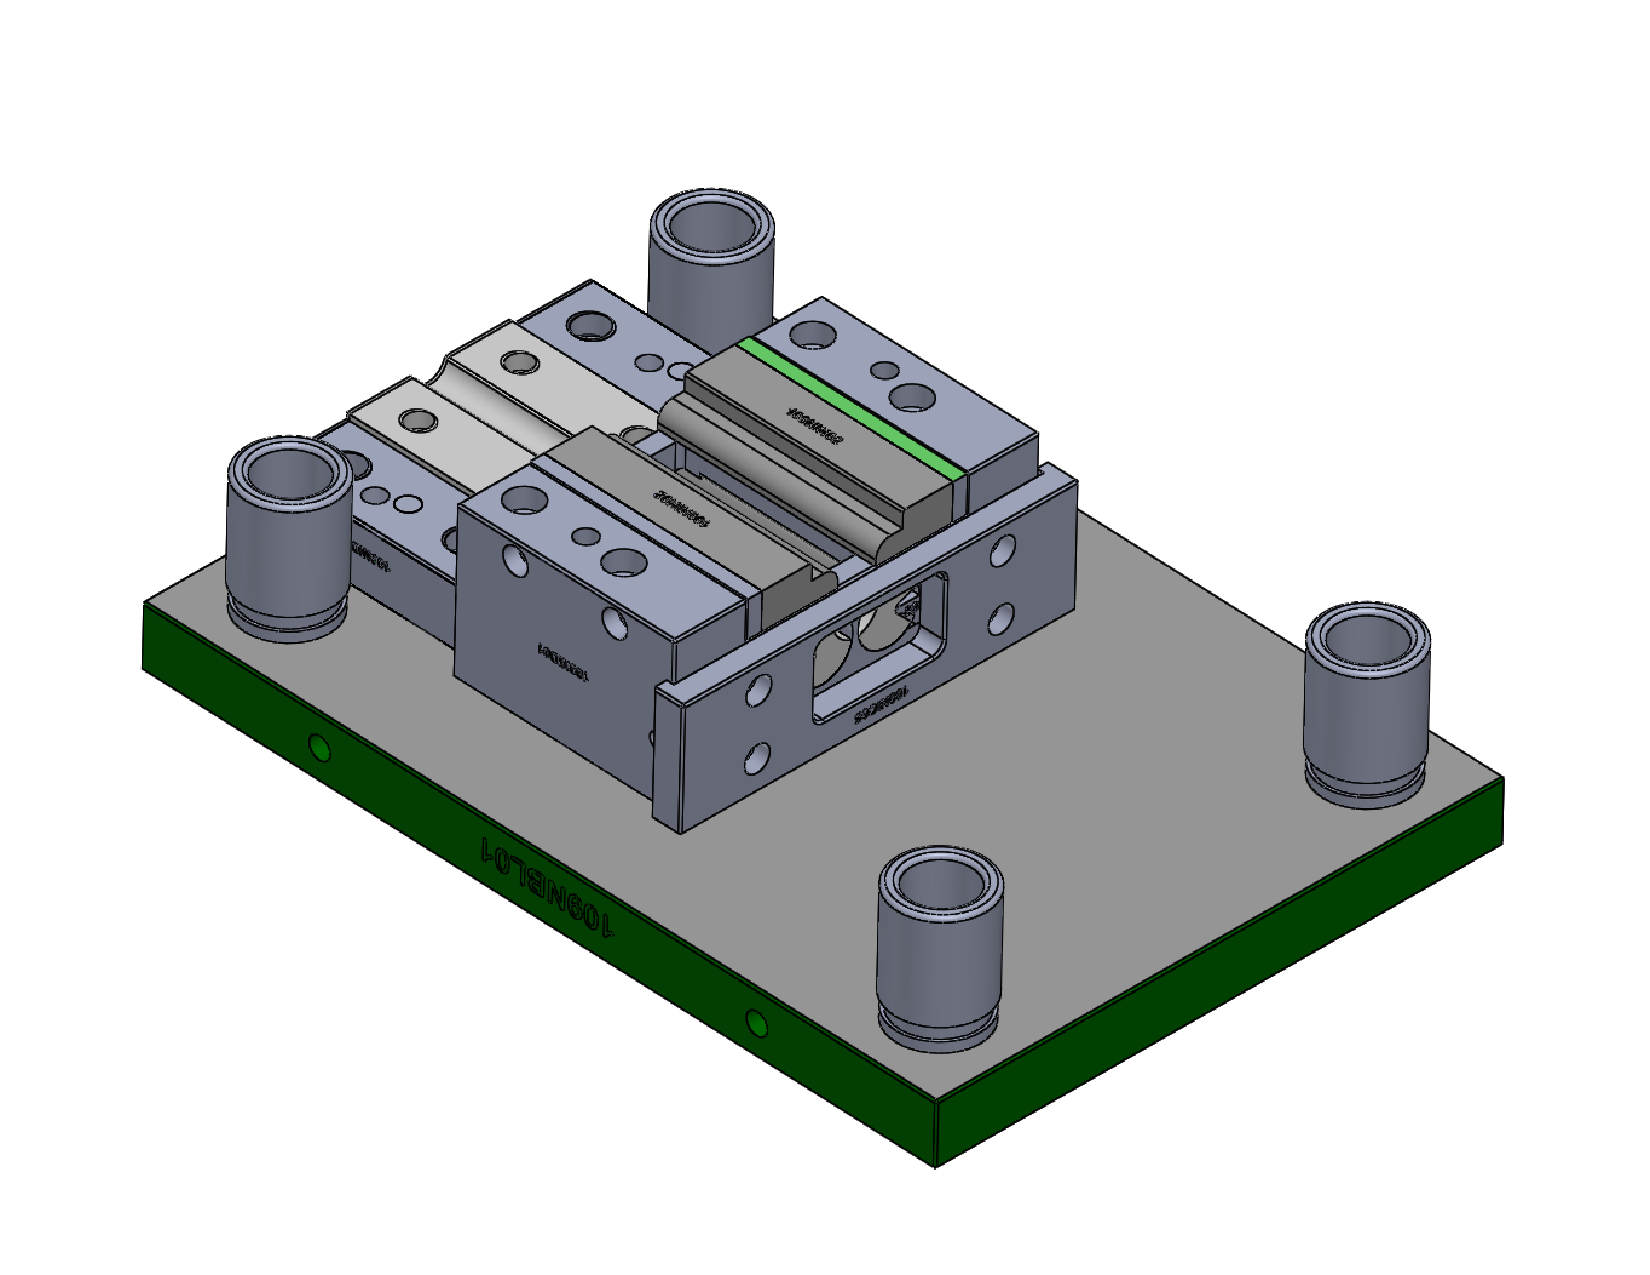
\includegraphics[width=\textwidth]{src/ch3/troquel_vista_superior.pdf}
    \caption{}
    \label{fig:troquel_vista_superior}
\end{subfigure}
\caption{Partes a) inferior y b) superior del troquel}

\end{figure}


\subsection{Generalidades de la simulación}



\subsection{Modelo constitutivo}

Para la pieza de trabajo se utilizó un modelo de tipo \textit{Piecewise Linear Plasticity}, 
el cual es un modelo multilineal que permite utilizar una curva esfuerzo-deformación y la 
dependencia de la tasa de deformación como datos de entrada para definir el comportamiento 
plástico del material. Para cuantificar la tasa de deformación este modelo utiliza la 
relación de Cowper-Symonds mostrada en la ecuación \ref{eq:cowper_symonds}.\\

\begin{equation} \label{eq:cowper_symonds}
\sigma_{y}\left( \varepsilon _{eff}^{P},\dot{\varepsilon }_{eff}^{P} \right) = 
{{\sigma }_{y}}\left( \varepsilon _{eff}^{P} \right)\left[ 1+{{\left( \frac{\dot{\varepsilon }_{eff}^{P}}{C} \right)}^{\frac{1}{P}}} \right]
\end{equation}

La curva esfuerzo-deformación ingresada en el software de simulación fue la obtenida 
de forma experimental, con algunas modificaciones a saber: se tomaron solamente 7 puntos 
de la curva original linealmente equiespaciados, se calculó el esfuerzo y deformación verdadera 
mediante las ecuaciones descritas en la sección \ref{subsec:true_strain_stress}, posteriormente 
a partir de la deformación verdadera se obtuvo la deformación plástica mediante la 
ecuación \ref{eq:plastic_strain}, mismas que se agrupan en la tabla \ref{tab:strain_stress_conversion}.
La curva resultante y que se ingresó en el softaware se muestra en la figura \ref{fig:ls_dyna_material_curve}. \\

Para definir completamente el modelo es necesario asignar las propiedades mecánicas elementales 
como el módulo elástico, la relación de Poisson y la densidad. Además, se debe asignar 
la resistencia a la fluencia y las constantes C y P utilizadas en la ecuación de Cowper-Symonds.
Estas propiedades utilizadas se muestran en la tabla \ref{tab:material_properties}. \\

% Tabla de propiedades
\begin{table}[h]
\centering
\caption{Propiedades del acero AISI 1018}
\label{tab:steel_properties}
\begin{tabular}{p{4cm} p{4cm}} \hline
Propiedad & Magnitud (unidades) \\
\hline
Módulo elástico & 29 000 (ksi) \\
Densidad & 0.00073 (lbf s$^2$/in$^4$) \\
Esfuerzo de fluencia & 52 000 (psi) \\
Coeficiente de Poisson & 0.3 \\
C & 40 (s$^{-1}$) \\
P & 5 \\
\hline
\end{tabular}
\label{tab:material_properties}
\end{table}

En los componentes del troquel se utilizó un modelo rígido, para el cual sólo es necesario 
especificar las propiedades elásticas. Los componentes rígidos, normalmente, permiten la 
aplicación de condiciones de desplazamiento utilizando el identificador o ID de la parte, además 
se pueden asignar propiedades de inercia o velocidades iniciales. En este caso, no se 
especificaron propiedades adicionales, lo cual implica que el software de simulación calcule automáticamente 
las propiedades inerciales basadas en el modelo de elemento finito. \\

Para crear los materiales de cada uno de los componentes se utilizó un pequeño \textit{script}, 
que se muestra a continuación:

\begin{apdl}
! Para el formador inferior
MP,EX,2,29E6 ! psi
MP,NUXY,2,0.3 ! 
MP,DENS,2,0.00073 ! lbf s^2 / in^4
EDMP,rigid,2,7,7

! Formador superior izquierdo
MP,EX,3,29E6 ! psi
MP,NUXY,3,0.3 ! 
MP,DENS,3,0.00073 ! lbf s^2 / in^4
EDMP,rigid,3,6,7

! Formador superior derecho
MP,EX,4,29E6 ! psi
MP,NUXY,4,0.3 ! 
MP,DENS,4,0.00073 ! lbf s^2 / in^4
EDMP,rigid,4,6,7

! Leva izquierda
MP,EX,5,29E6 ! psi
MP,NUXY,5,0.3 ! 
MP,DENS,5,0.00073 ! lbf s^2 / in^4
EDMP,rigid,5,6,4

! Leva derecha
MP,EX,6,29E6 ! psi
MP,NUXY,6,0.3 ! 
MP,DENS,6,0.00073 ! lbf s^2 / in^4
EDMP,rigid,6,6,4

! Para el blank
! Propiedades elásticas
MP,EX,1,29E6 ! psi
MP,NUXY,1,0.3 ! 
MP,DENS,1,0.00073 ! lbf s^2 / in^4

! Definir un arreglo para la deformación plástica verdadera
*dim,strn,,6
! Definir un arreglo para el esfuerzo verdadero
*dim,strs,,6

! Deformación (in/in)
strn(1) = 0.0, 0.0293, 0.0772, 0.1562, 0.2356, 0.344943

! Esfuerzo (psi)
strs(1) = 52489.4,60585.8,70710,76809.3,80244.3,82574.1

! Curva #1: Abscisa=deformación & Ordenada=esfuerzo
edcurve,add,1,strn,strs 

! Especificar Power Law #8 para el material #1
TB,PLAW,1,,,8  ! Piecewise Linear Plasticity

! Usar curva #1 para la relación esfuerzo-deformación
TBDATA,1,52e3 ! Esfuerzo de fluencia (psi)
TBDATA,3,.75 ! Deformación de falla
TBDATA,4,40.0 ! C (Parámetro de tasa de deformación)
TBDATA,5,0.1 ! P (Parámetro de tasa de deformación)
TBDATA,6,1 ! ID de la curva
\end{apdl}


% Tabla de propiedades plásticas

\begin{table}[h]
\centering
\caption{Conversión de esfuerzos y deformaciones}
\label{tab:strain_stress_conversion}
\begin{tabular}{p{2.5cm} p{2.5cm} p{2.5cm} p{2.5cm} p{2.5cm}} \hline
{\bf $\varepsilon_{nom}$ & $\sigma_{nom}$ (psi) & $\varepsilon_t$ & $\sigma_t$ (psi) & $\varepsilon_{pl}$ } \\
\hline
0.0084 & 51376.41 & 0.0084 & 51808.49 & 0.0000 \\
0.0224 & 59624.27 & 0.0221 & 60957.47 & 0.0200 \\
0.0418 & 67059.05 & 0.0409 & 69858.77 & 0.0385 \\
0.0607 & 70769.55 & 0.0589 & 75063.85 & 0.0563 \\
0.0846 & 72814.73 & 0.0812 & 78971.94 & 0.0785 \\
0.1287 & 72924.09 & 0.1210 & 82305.77 & 0.1182 \\
0.1554 & 70462.94 & 0.1444 & 81412.18 & 0.1416 \\
\hline
\end{tabular}
\label{tab:stress_strain_curve}
\end{table}


\begin{center}
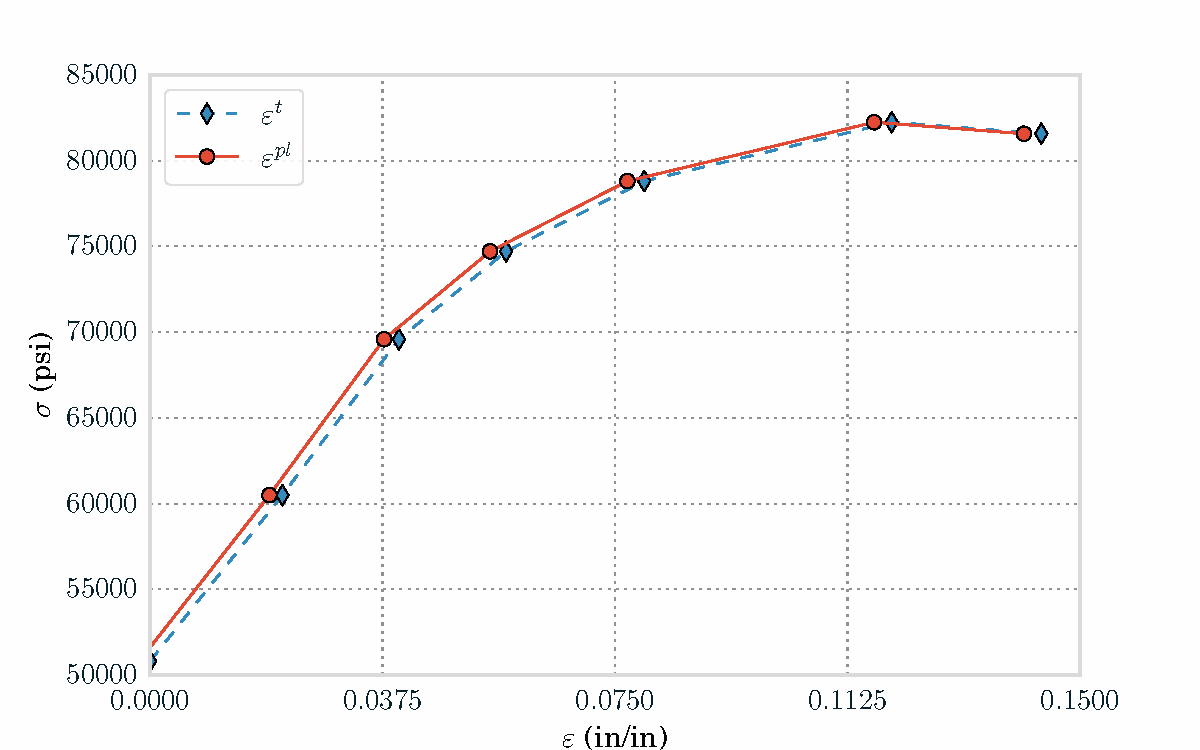
\includegraphics[scale=0.6]{src/ch3/ls_dyna_material_curve.pdf}
\captionof{figure}{Curva esfuerzo-deformación ingresada en ANSYS/LS-DYNA}
\label{fig:ls_dyna_material_curve}
\end{center}


\subsection{Mallado}

\subsubsection{Primer ensamble}

Para el mallado de la pieza de trabajo se utilizó el elemento \texttt{SOLID164} 
( ver figura \ref{fig:solid164} ), el cual es un sólido de 8 nodos, que puede ser utilizado con el modelo 
constitutivo descrito en la sección anterior. Este elemento utiliza, por defecto, integración reducida 
(un punto de integración), el cual tiene la ventaja de reducir el tiempo de cómputo y adiciona 
robustez para el caso de grandes deformaciones ~\cite{lsdyna-ansys-manual}, no obstante puede presentar 
la desventaja de propiciar la inclusión de los modos de Hourglass en la solución, implicando que 
se obtenga una malla deformada con apariencia corrugada.

\begin{center}
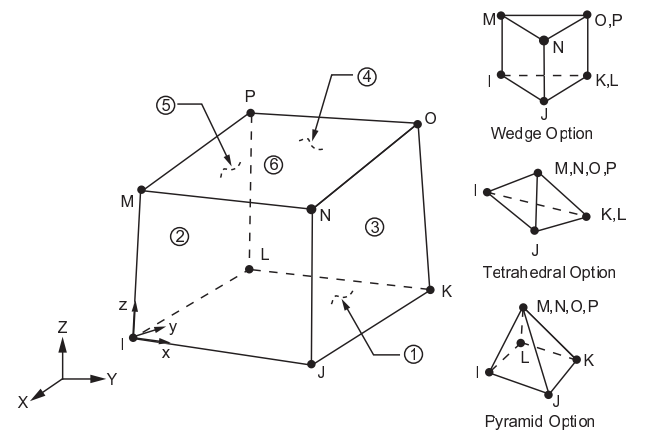
\includegraphics[scale=0.65]{src/ch3/solid164.png}
\captionof{figure}{Elemento \texttt{SOLID164}}
\label{fig:solid164}
\end{center}

En los componentes del troquel se mallaron solamente las áreas que están en contacto directo con el 
\textit{blank} durante el proceso de formado, con la finalidad de reducir el número de elementos del modelo. 
Se utilizaron elementos \texttt{SHELL163} para realizar el mallado. Los parámetros requeridos para 
este elemento se indican en la tabla \ref{tab:shell_param}.

\begin{center}
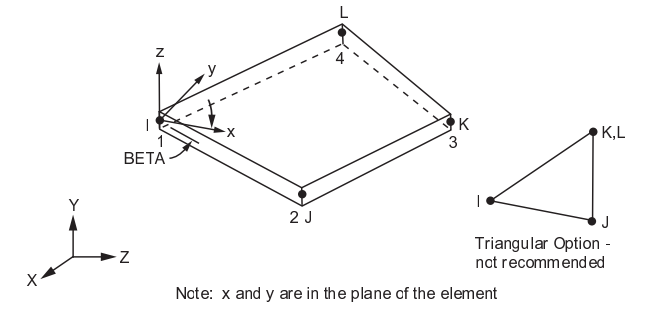
\includegraphics[scale=0.65]{src/ch3/shell163.png}
\captionof{figure}{Elemento SHELL163}
\label{fig:shell163}
\end{center}


% Tabla de propiedades para elemento SHELL163
\begin{table}[h]
\centering
\caption{Parámetros utilizados para el elemento SHELL163}
\label{}
\begin{tabular}{p{6cm} p{6cm}} \hline
Parámetros & Valores \\
\hline
General shell formulation & Belytschko-Tsay \\
Membrane element formulation & Belytschko-Tsay Membrane \\
Triangular shell formulation & $C^0$ triangular shell \\
\hline
\end{tabular}
\label{tab:shell_param}
\end{table}


% Tabla de constantes reales para elemento SHELL163
\begin{table}[h]
\centering
\caption{Constantes reales para el elemento SHELL163}
\label{}
\begin{tabular}{p{6cm} p{3cm}} \hline
Parámetros & Valores \\
\hline
Factor cortante (SHRF) & 5/6 \\
Puntos de integración (NIP) & 1 \\
Espesor en nodo 1 (T1) & 0.2 \\
Espesor en nodo 2 (T2) & 0.2 \\
Espesor en nodo 3 (T3) & 0.2 \\
Espesor en nodo 4 (T4) & 0.2 \\
\hline
\end{tabular}
\label{tab:shell_param}
\end{table}


En el \textit{blank} se utilizó un tamaño global de elemento de 0.03 in, y 0.035 in en el caso de las partes 
rígidas, exceptuando las áreas que están directamente en contacto con el \textit{blank}, en cuyo caso se hizo 
un refinamiento, dejando el tamaño global en 0.02 in. En el \textit{blank} fue necesario segmentar en cuatro 
volúmenes, para permitir un mallado más uniforme (ver figura \ref{fig:blank_seg} ).


% Partición del blank
\begin{center}
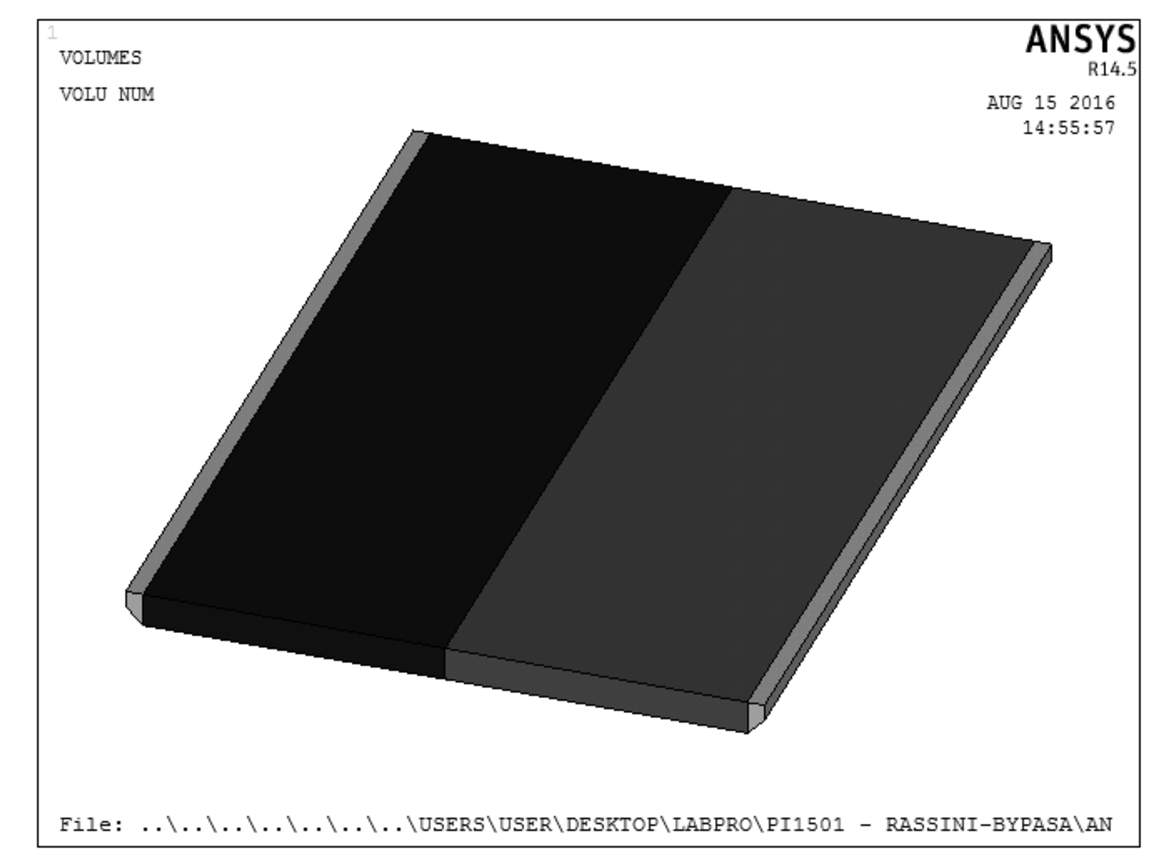
\includegraphics[width=0.5\textwidth]{src/ch3/blank_segmentado.pdf}
\captionof{figure}{Blank segmentado en cuatro regiones}
\label{fig:blank_seg}
\end{center}


% Mallado del blank


\begin{figure}[!h]
\centering
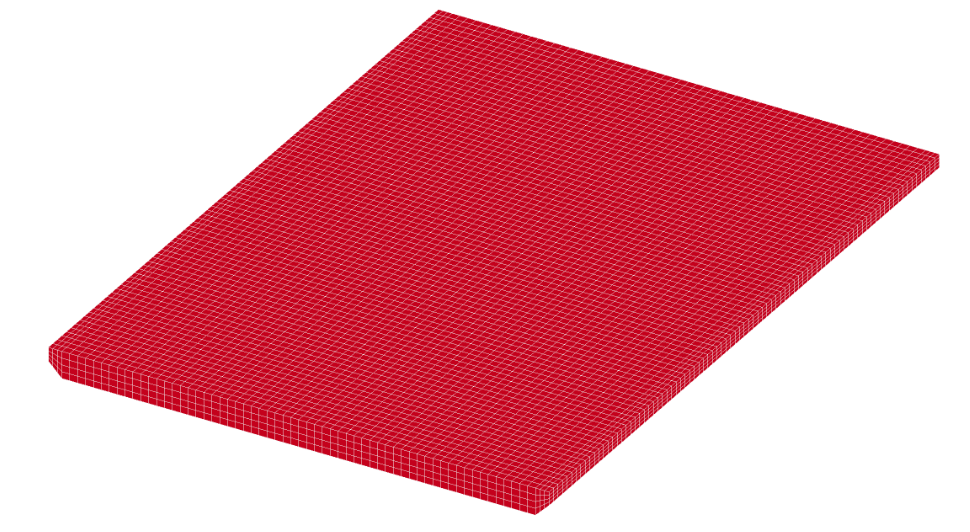
\includegraphics[width=0.5\textwidth]{src/ch3/mesh_blank.png}
\label{fig:mesh_blank}
\caption{Mallado del blank}
\end{figure}


\begin{figure}[!h]
\centering
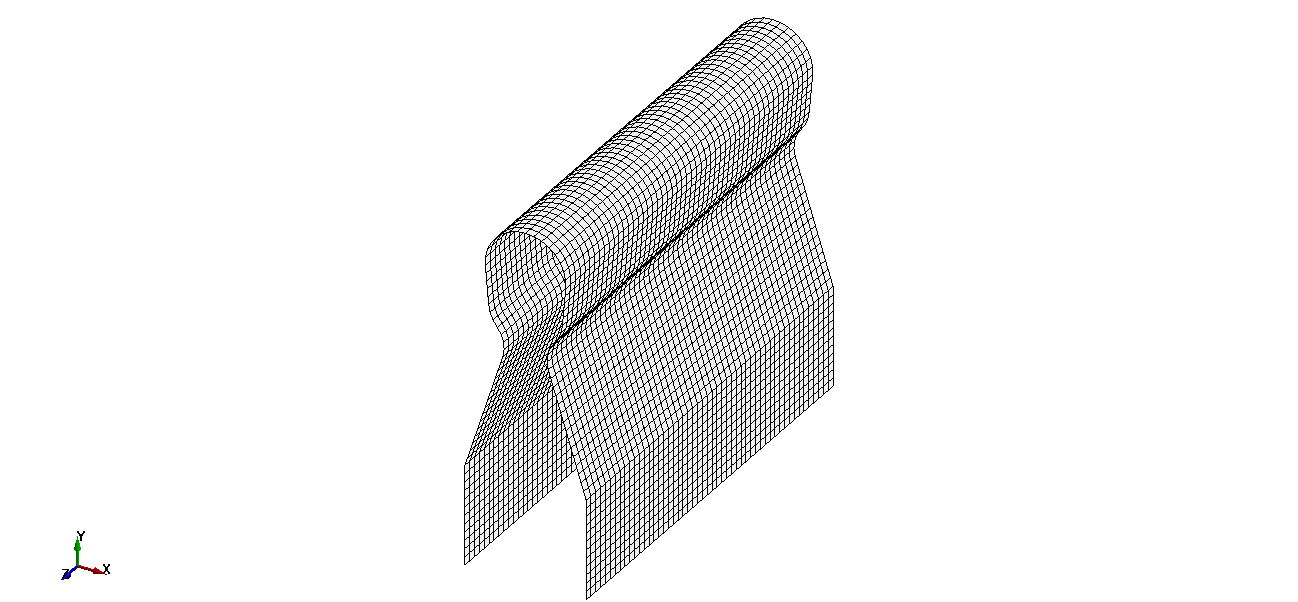
\includegraphics[width=0.5\textwidth]{src/ch3/mesh_fi.png}
\caption{Mallado del formador inferior}
\label{fig:mesh_fi}
\end{figure}

\begin{figure}[!h]
\centering
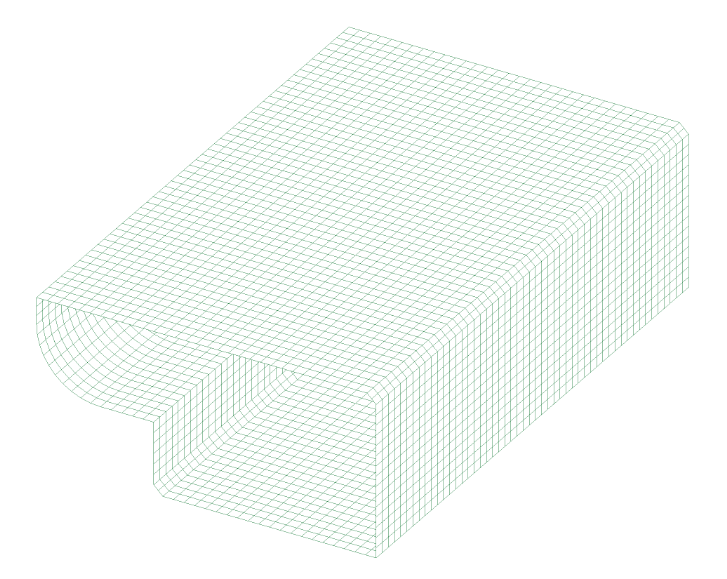
\includegraphics[width=0.5\textwidth]{src/ch3/mesh_fs.png}
\caption{Mallado del formador superior}
\label{fig:mesh_fi}
\end{figure}

\begin{figure}[!h]
\centering
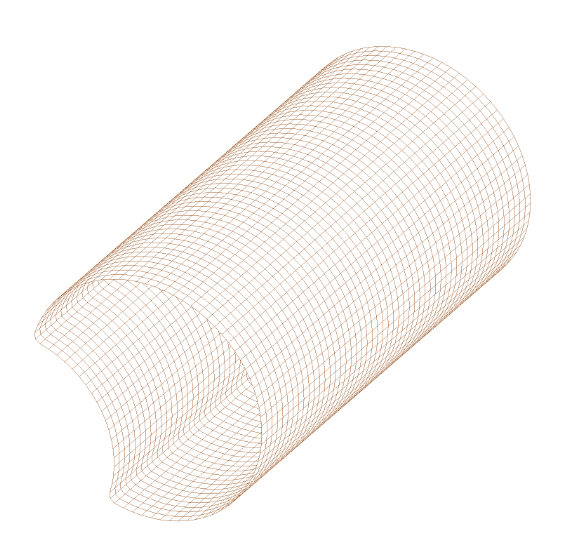
\includegraphics[width=0.5\textwidth]{src/ch3/mesh_leva.png}
\caption{Mallado de la leva}
\label{fig:mesh_fi}
\end{figure}


% \begin{figure}[!h]
% \centering
% \begin{subfigure}[t]{0.3\textwidth}
% \centering
% 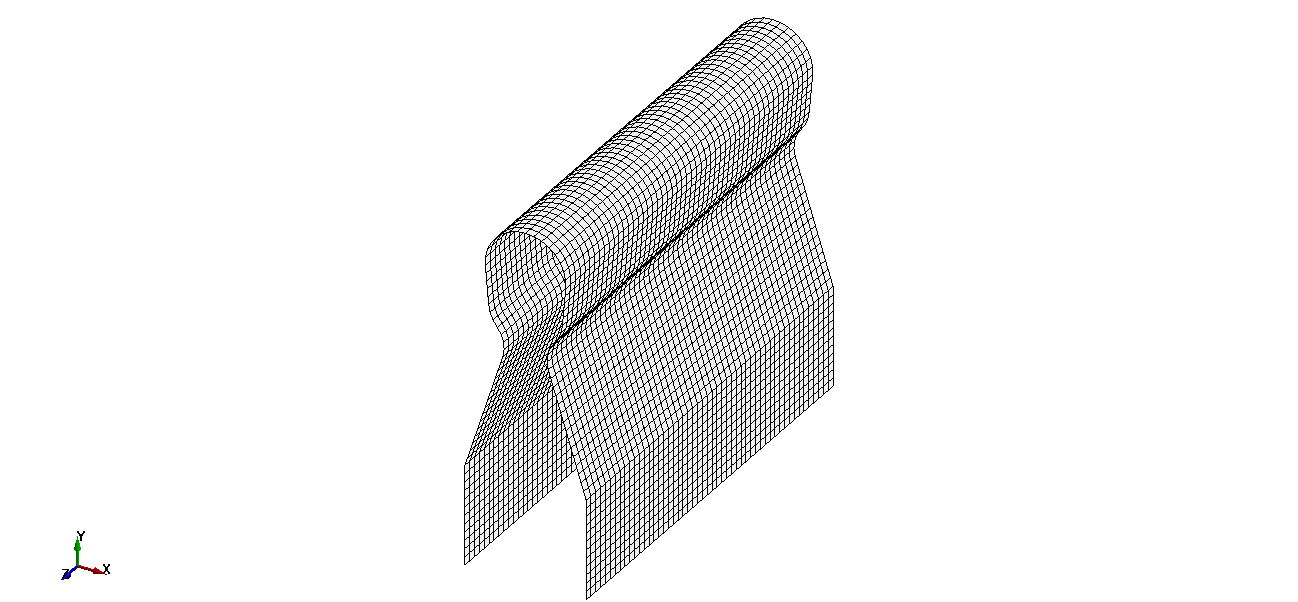
\includegraphics[width=\textwidth]{src/ch3/mesh_fi.png}
% \caption{}
% \label{fig:mesh_fi}
% \end{subfigure}
% ~ 
% \begin{subfigure}[t]{0.3\textwidth}
% \centering
% 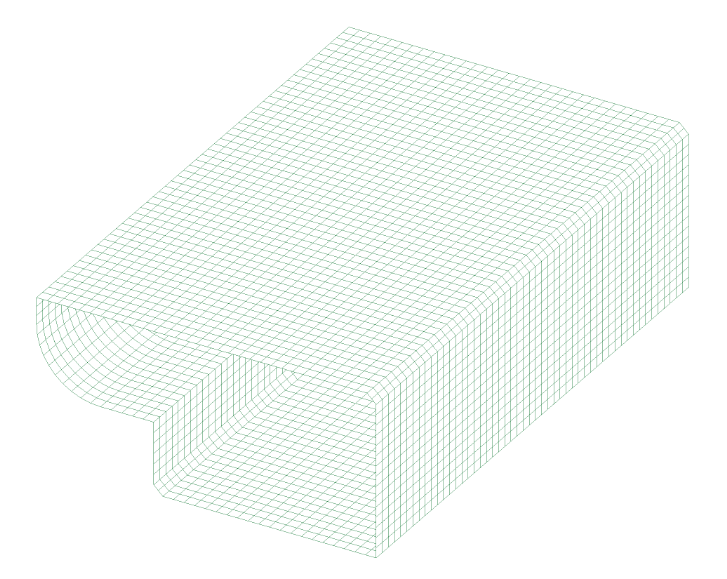
\includegraphics[width=\textwidth]{src/ch3/mesh_fs.png}
% \caption{}
% \label{fig:mesh_fs}
% \end{subfigure}
% ~ 
% \begin{subfigure}[t]{0.3\textwidth}
% \centering
% 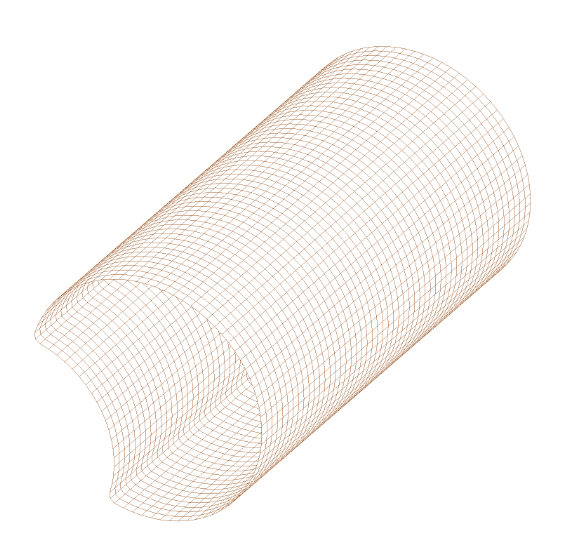
\includegraphics[width=\textwidth]{src/ch3/mesh_leva.png}
% \caption{}
% \label{fig:mesh_leva}
% \end{subfigure}

% \caption{Mallado de a) formador inferior b) formador superior c) leva}
% \end{figure}


%  Partes 
\begin{figure}[!h]
\centering
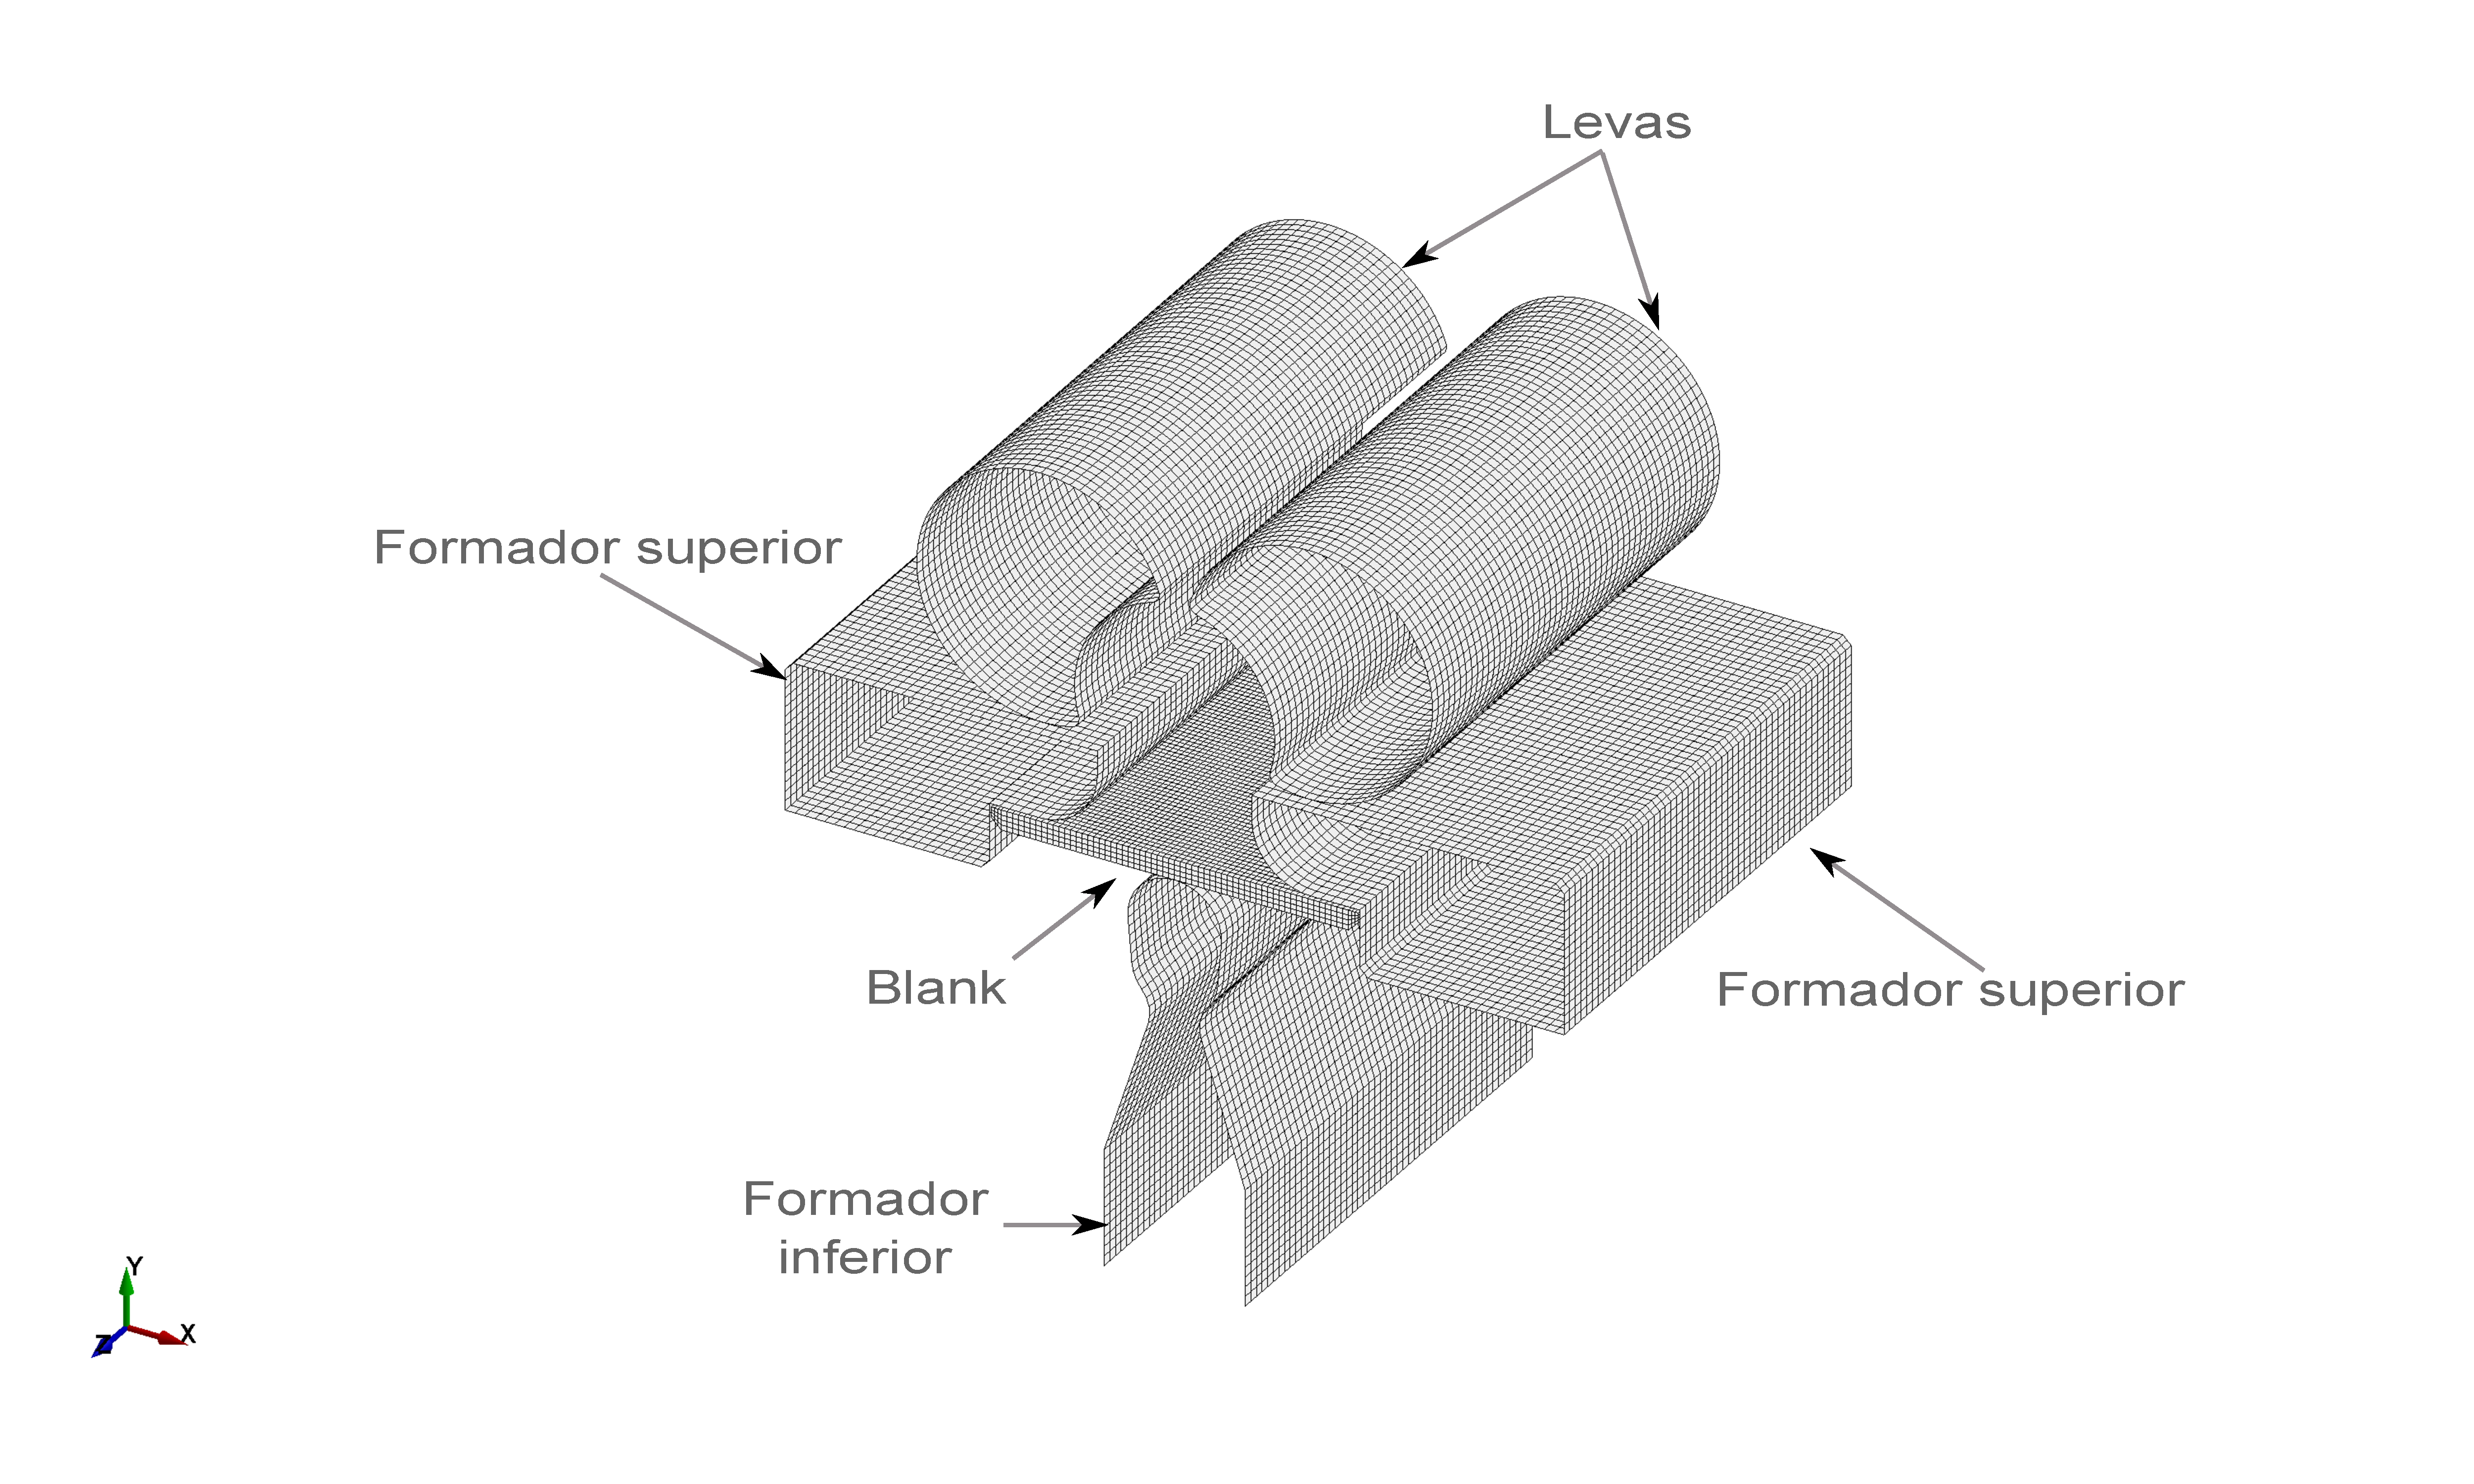
\includegraphics[width=0.8\textwidth]{src/ch3/parts_01.pdf}
\caption{Partes del ensamble 1}
\label{fig:parts_01}
\end{figure}

% En las tabla \ref{tab:elements_and_nodes} se muestra el número de nodos y elementos obtenidos 
% para cada uno de los ensambles.

% \begin{table}[h]
% \centering
% \caption{Número de nodos y elementos}
% \label{}
% \begin{tabular}{p{2cm} p{2cm} p{2cm}} \hline
%  & Nodos & Elementos \\
% \hline
% Paso 1 & 52285 & 45348 \\
% Paso 2 & 48884 & 42264 \\
% \hline
% \end{tabular}
% \label{tab:elements_and_nodes}
% \end{table}


\subsubsection{Segundo ensamble}

Al igual que en el primer ensamble, los formadores y/o componentes del herramental, se 
mallaron por áreas utilizando elementos \texttt{SHELL163}. En el caso de la pieza de trabajo, 
esta se importó en su configuración deformada del análisis del primer paso, incluyendo 
además la distribución de esfuerzos. En la figura \ref{fig:mesh_blank_02} se observa 
la malla deformada del blank. El mallado de cada uno de los componentes del troquel 
se puede observar en las figuras \ref{fig:mesh_ffi}, \ref{fig:mesh_ffs} y \ref{fig:mesh_perno}.


\begin{figure}[!h]
\centering
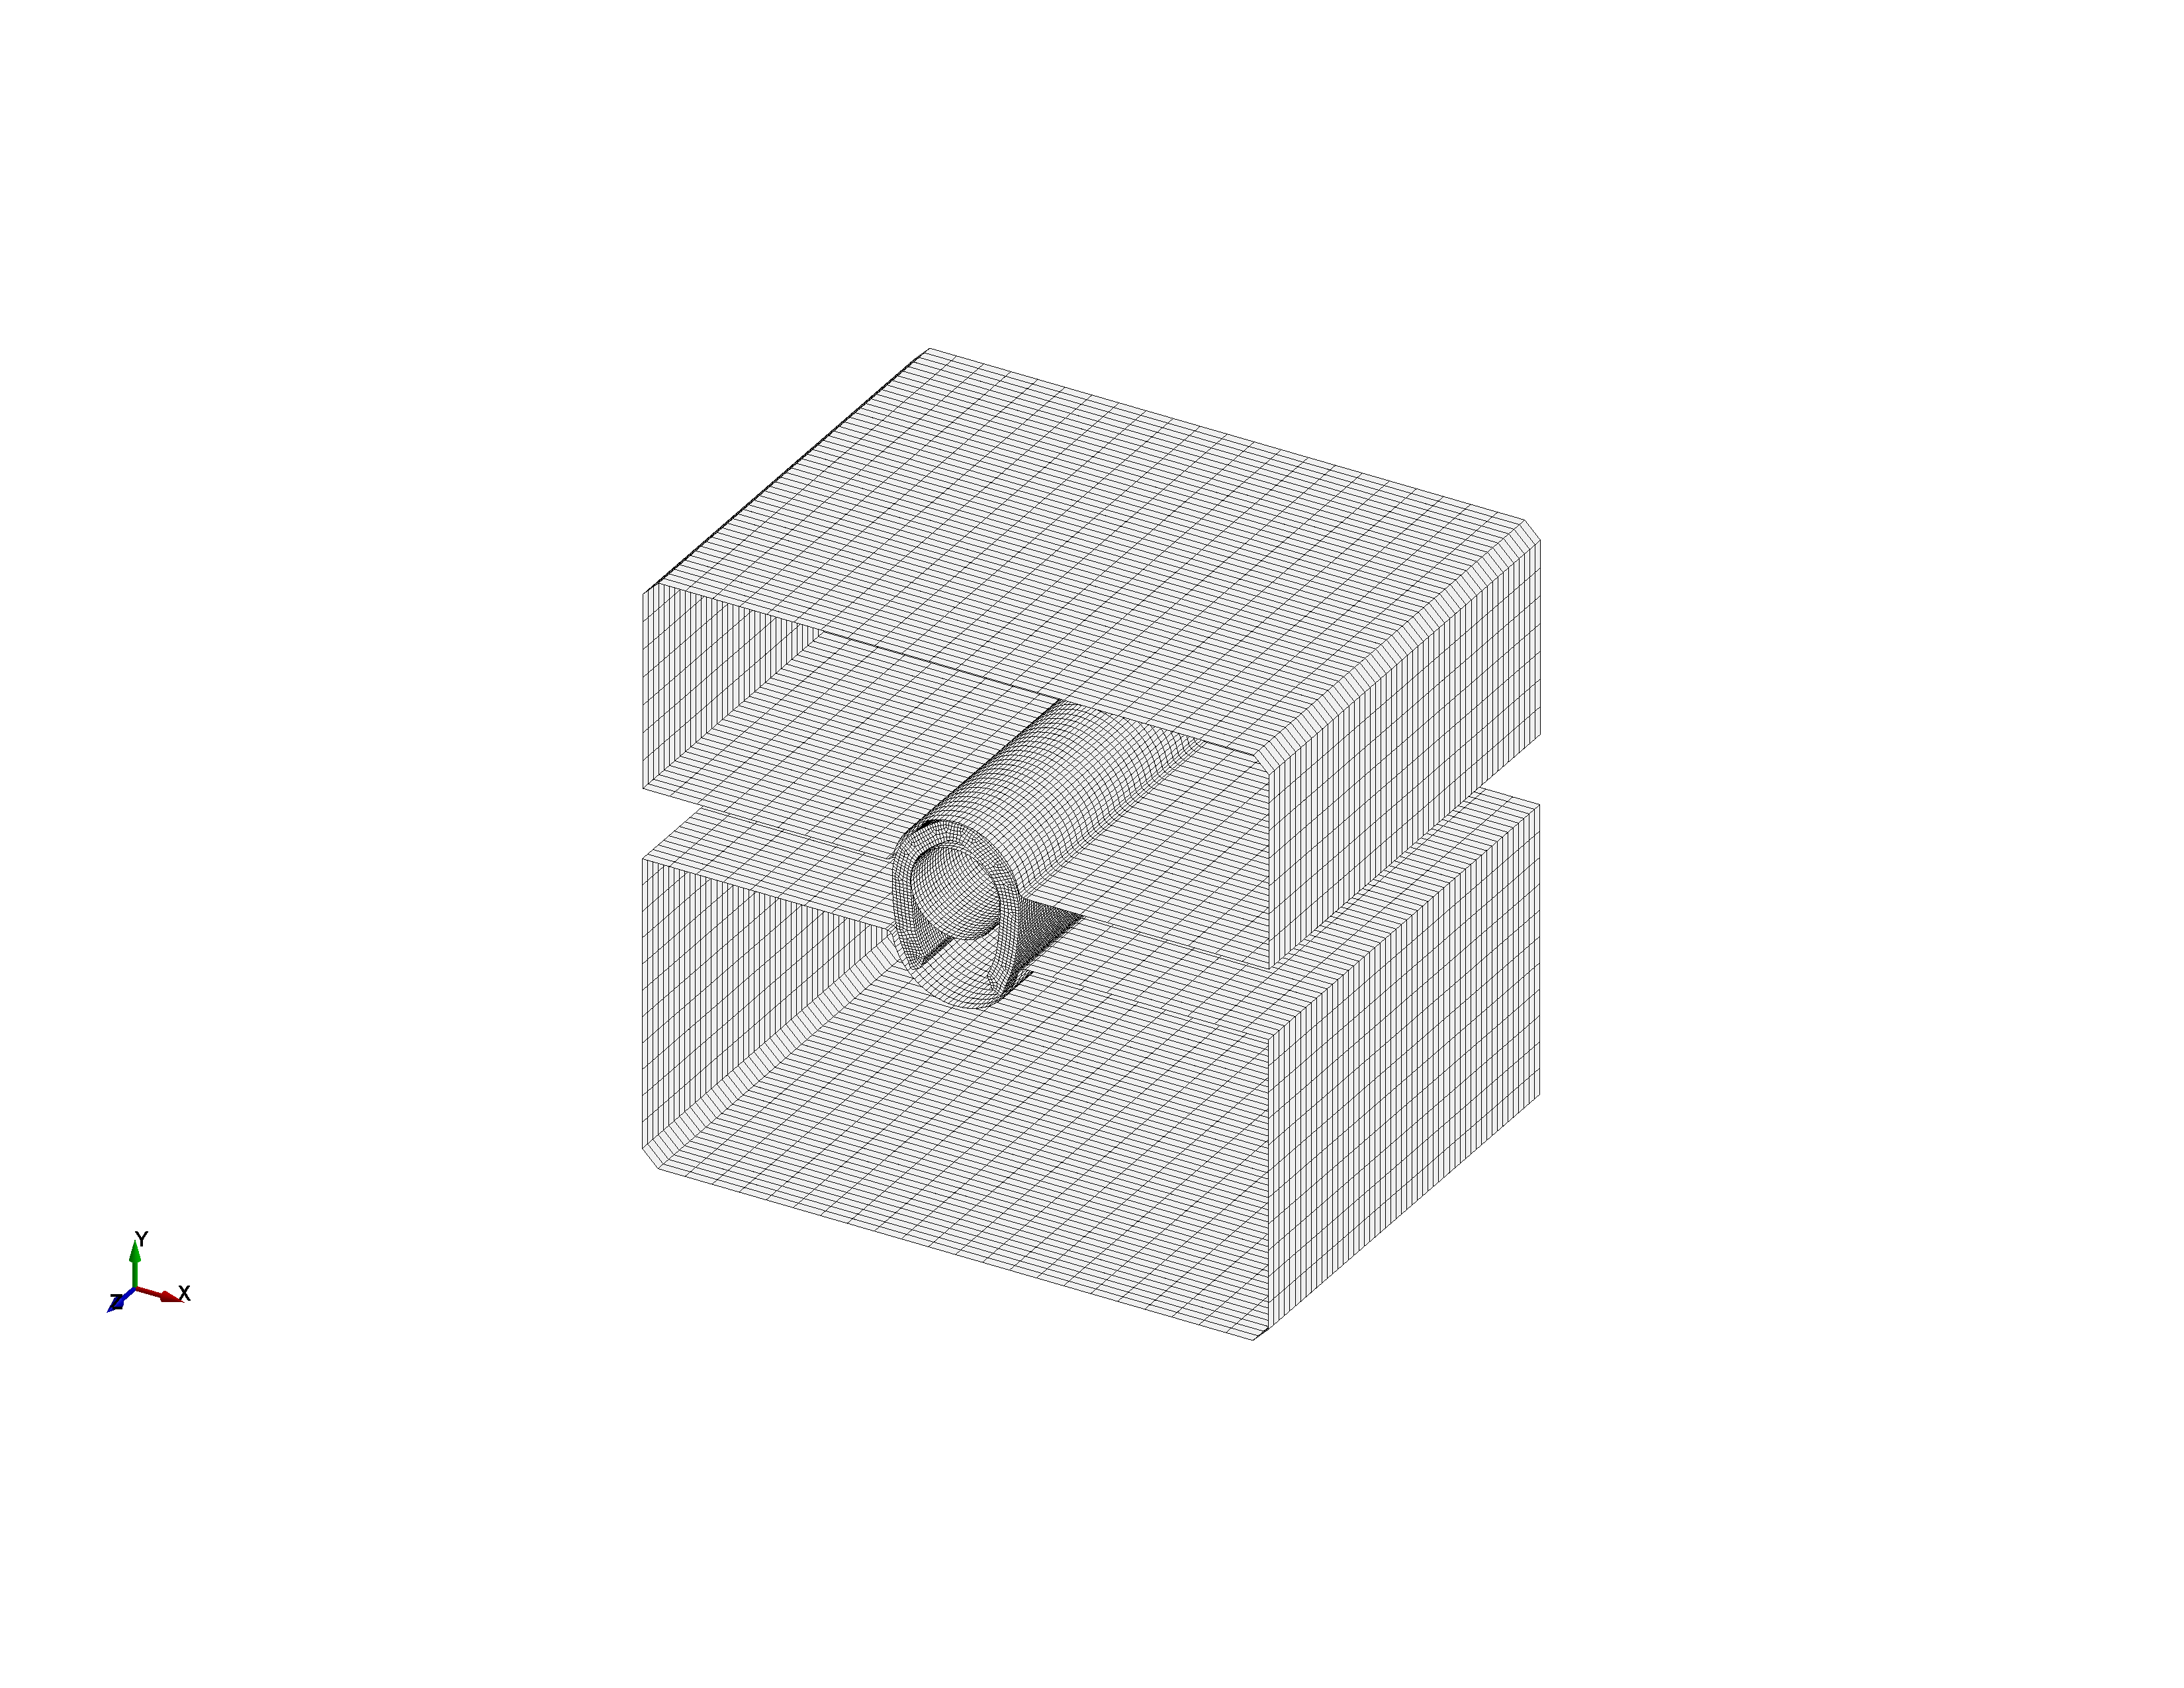
\includegraphics[width=0.6\textwidth]{src/ch3/parts_02.png}
\caption{Mallado del segundo ensamble}
\label{fig:parts_02}
\end{figure}

\begin{figure}[!h]
\centering
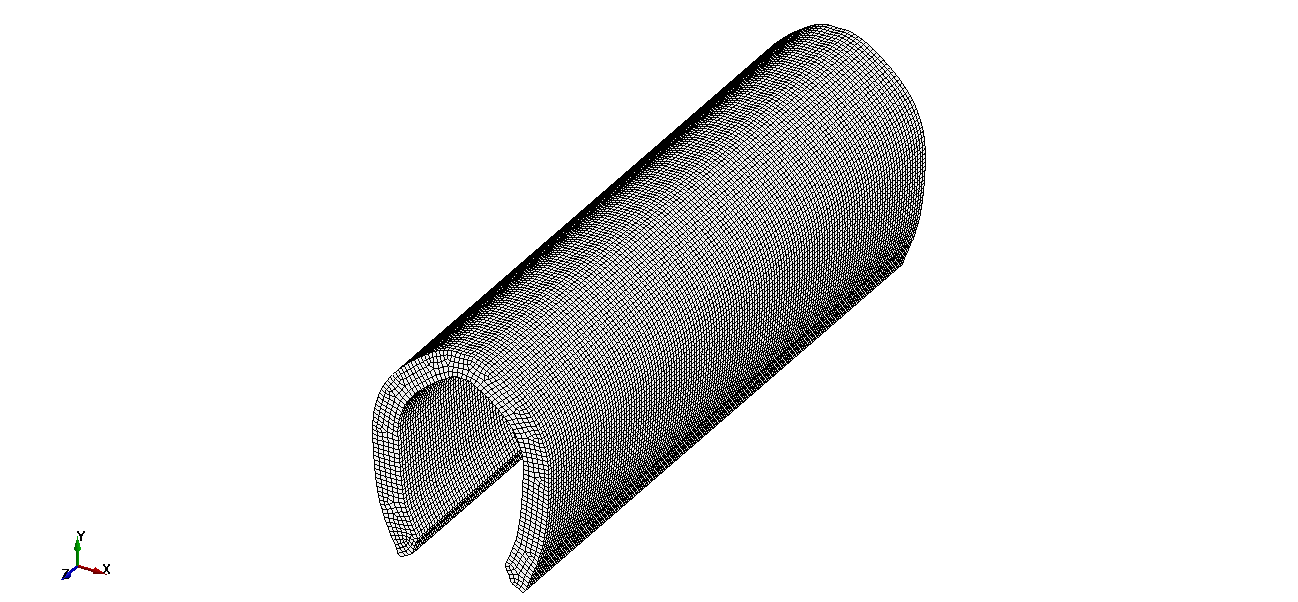
\includegraphics[width=0.5\textwidth]{src/ch3/mesh_blank_02.png}
\caption{Geometría deformada del blank importada del primer paso}
\label{fig:mesh_blank_02}
\end{figure}

\begin{figure}[!h]
\centering
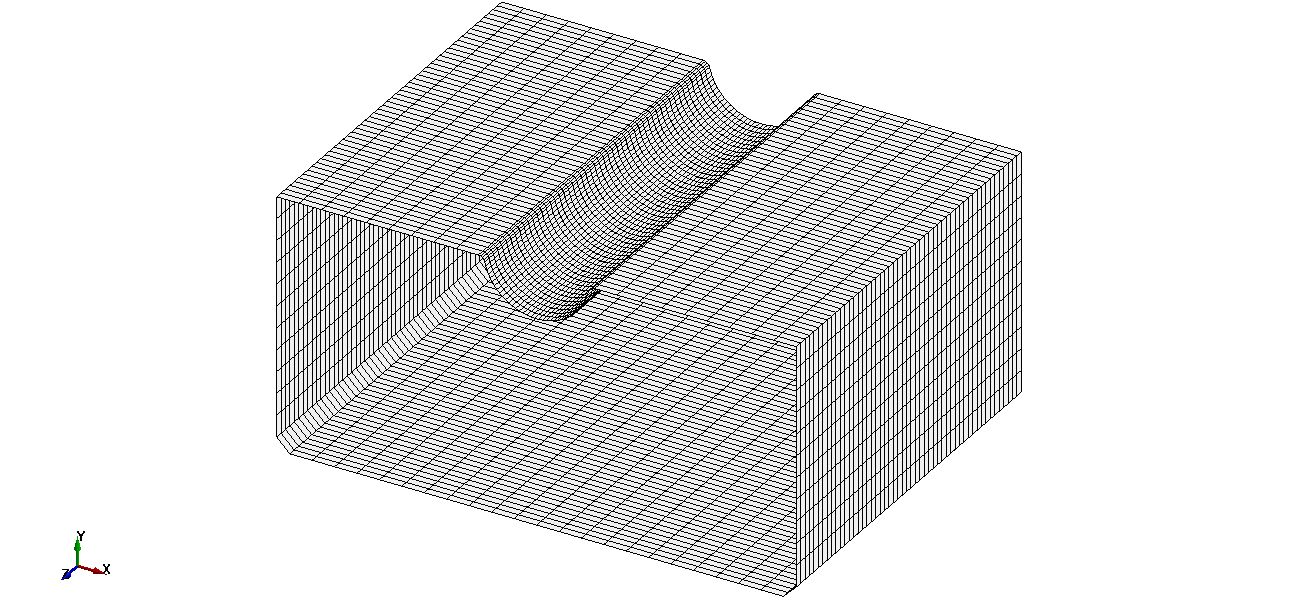
\includegraphics[width=0.5\textwidth]{src/ch3/mesh_ffi.png}
\caption{Mallado del formador final inferior}
\label{fig:mesh_ffi}
\end{figure}

\begin{figure}[!h]
\centering
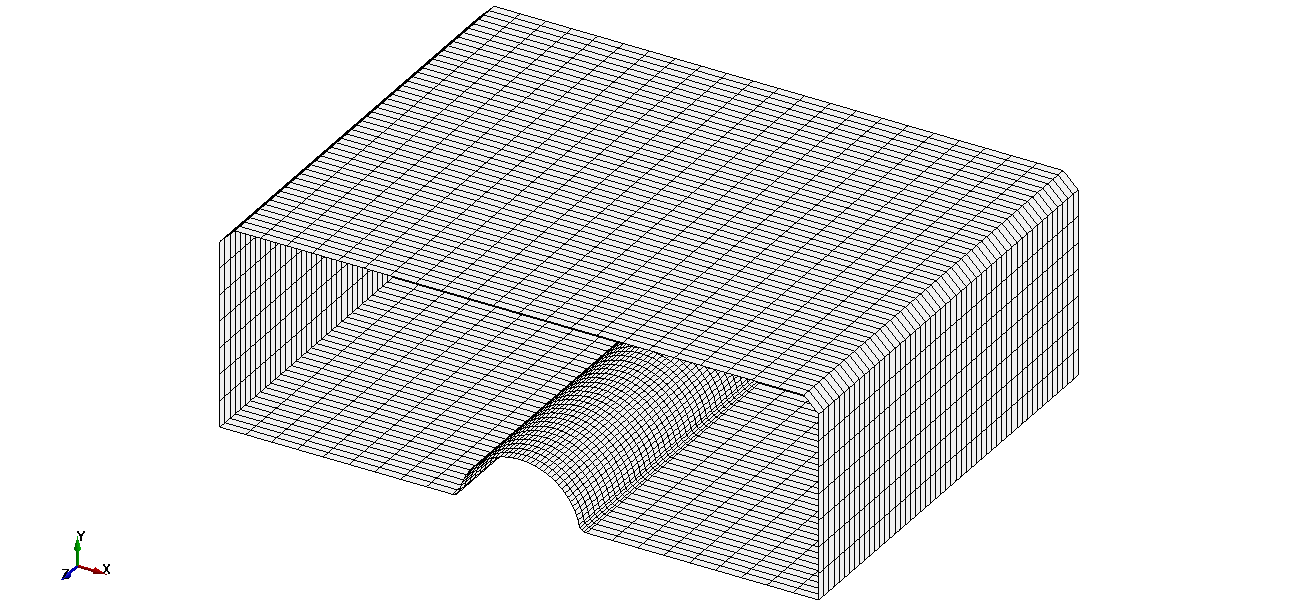
\includegraphics[width=0.5\textwidth]{src/ch3/mesh_ffs.png}
\caption{Mallado del formador final superior}
\label{fig:mesh_ffs}
\end{figure}

\begin{figure}[!h]
\centering
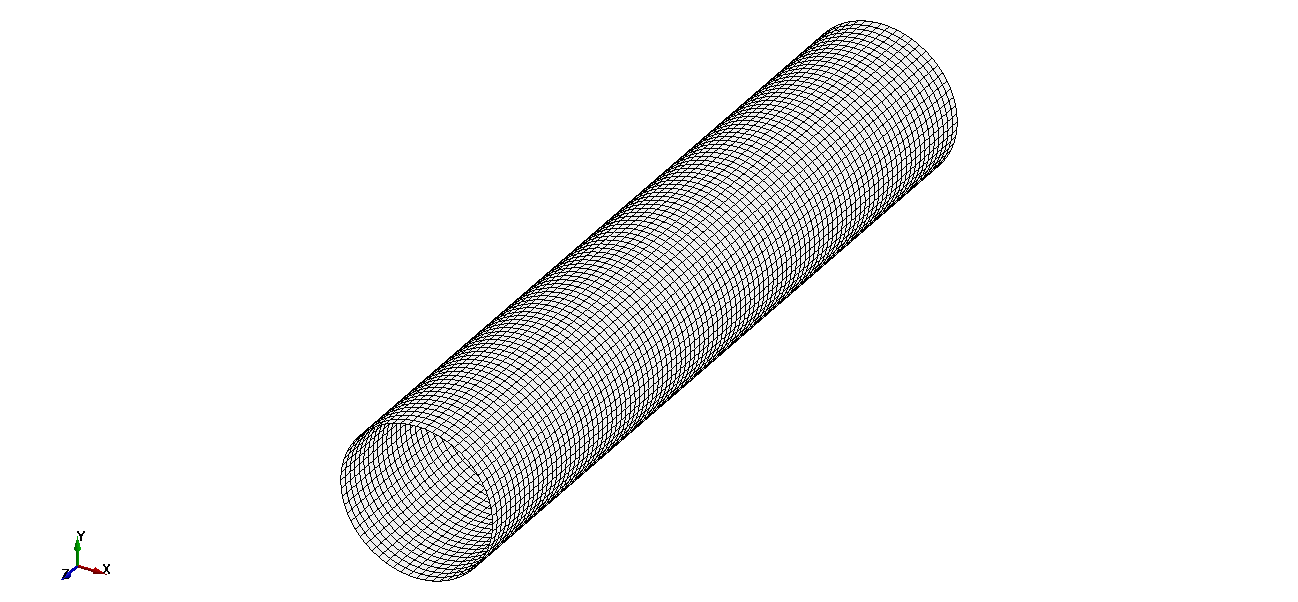
\includegraphics[width=0.5\textwidth]{src/ch3/mesh_perno.png}
\caption{Mallaod del perno formador}
\label{fig:mesh_perno}
\end{figure}


% Condiciones de frontera ==================================================================
\subsection{Condiciones de frontera}

Para efectos de la simulación el blank fue sujetado en el punto medio de cada extremo, 
en las direcciones \textit{X} y \textit{Z}, para evitar que se desplace de manera no 
deseada y con esto ayudar en la convergencia de la solución. La localización de las 
condiciones de sujeción en la parte central se debe a que se considera que la placa 
no sufre una deformación significativa en esa parte y por tanto no influirá en el campo 
de deformaciones resultante. \\

Los componentes del troquel, al ser cuerpos rígidos, la mayoría de sus 
restricciones fueron consideradas en la definición del material. En el caso de los 
formadores superiores, sólo se especificaron los desplazamientos en la dirección 
vertical Y, se utilizaron arreglos unidimensionales para especificar la relación
tiempo-desplazamiento, en todos los casos se especificó como desplazamiento de
cuerpo rígido en la dirección Y (\texttt{RBUY}), aplicándose esta condición a cada uno de los
componentes.\\

La relación tiempo-desplazamiento se definió utilizando una función de tipo
\textit{smooth-step}, cuya forma general es $f(t) = A(Bt^2 - Ct^3)$ , donde
$A$, $B$ y $C$ son constantes a ajustar para el requerimiento de desplazamiento total,
se caracteriza por tener un crecimiento lento al principio y final del intervalo
especificado, implicando una velocidad reducida de los formadores al principio y final 
del recorrido, con la finalidad de que esto facilite la estabilización y convergencia
del análisis.\\

En la figura \ref{fig:smooth_displacement_01} se muestra la gráfica del tiempo-desplazamiento 
utilizado en el primer paso del troquel. Para el segundo caso se utilizó una curva 
similar, con algunas variaciones en las constantes para disminuir la amplitud o valor máximo.\\


\begin{apdl}
*DIM,tiempo,ARRAY,400
*DIM,desplazamiento,ARRAY,400

*DO,ii,1,400
    tiempo(ii)=ii/2E3
*ENDDO

_k1 = 3.8E-7
_k2 = 1.15E-4
_k3 = -1.22

*DO,jj,1,200
    desplazamiento(jj)= _k3*(_k2*jj**2 - _k1*jj**3) - (_k3*(_k2 - _k1))
*ENDDO

*DO,kk,1,200
    desplazamiento(200+kk) = (-1)*_k3*(_k2*kk**2 - _k1*kk**3) + (_k3*(_k2*200**2 - _k1*200**3))
*ENDDO

*vplot,tiempo,desplazamiento
\end{apdl}


\begin{figure}[!h]
\centering
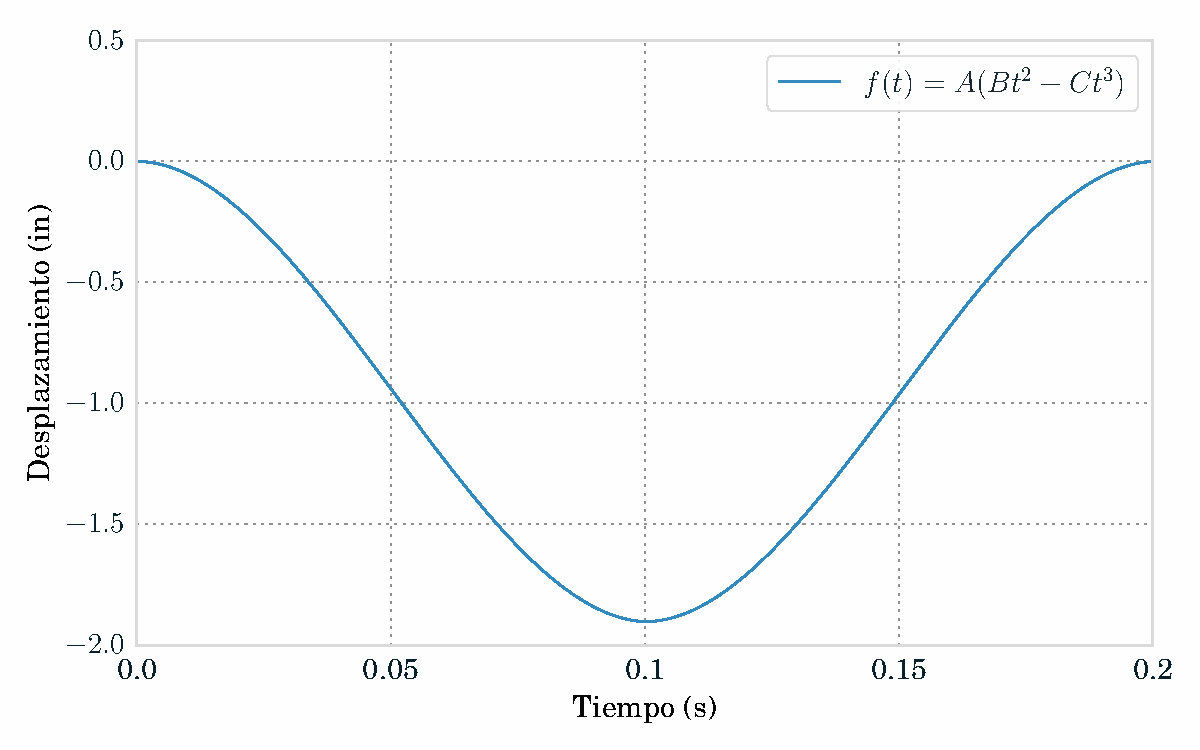
\includegraphics[scale=0.6]{src/ch3/smooth_displacement_01.pdf}
\captionof{figure}{Vector de tiempo desplazamiento}
\label{fig:smooth_displacement_01}
\end{figure}


% ==================================== CONTACTOS ============================================
\subsection{Contactos}

En la definición de contactos se utilizó un tipo de contacto superficie a superficie
general (\texttt{STS}). El programa de simulación utiliza los coeficientes de fricción 
estático ($FS$) y dinámico ($FD$) para la formulación del coeficiente friccional ($\mu_c$),
que viene dado por la ecuación :

\begin{equation}
\mu_c = FD + (FS - FD) e^{-DCv_{rel}}
\label{eq:frictional_coeff}
\end{equation}

Donde $DC$ es el coeficiente de decaimiento exponencial y $v_{rel}$ la velocidad relativa
entre las superficies en contacto ~\cite{lsdyna-manual}. Los valores del coeficiente de 
fricción estáticoy dinámico se establecieron en 0.2 y 0.1, respectivamente. ~\cite{carvill1993} \\

En la simulación del segundo paso se utilizó el contacto de tipo Single Surface (SS) para 
tomar en cuenta el contacto del blank con él mismo (cerrado del tubo) ~\cite{lsdyna-manual}, 
utilizandotambién los parámetros de fricción indicados anteriormente.

\section{Análisis experimental}

\texttt{EP-40-125TQ-350} 



